\documentclass[a4paper, 11pt, oneside, oldfontcommands]{memoir}

%%%%% Packages %%%%%
\usepackage{lmodern}
\usepackage{palatino}
\usepackage[T1]{fontenc}
\usepackage[utf8]{inputenc}
\usepackage[english]{babel}


%%%%%%%%%%%%%%%%%%%%  PACKAGE SECONDAIRE

%\usepackage{amstext,amsmath,amssymb,amsfonts} % package math
%\usepackage{multirow,colortbl}	% to use multirow and ?
%\usepackage{xspace,varioref}
\usepackage[linktoc=all, hidelinks]{hyperref}			% permet d'utiliser les liens hyper textes
\usepackage{float}				% permet d ajouter d autre fonction au floatant
%\usepackage{wrapfig}			% permet d avoir des image avec texte coulant a cote
%\usepackage{fancyhdr}			% permet d inserer des choses en haut et en bas de chaque page
\usepackage{microtype}			% permet d ameliorer l apparence du texte
\usepackage[explicit]{titlesec}	% permet de modifier les titres
\usepackage{graphics}			% permet d utiliser les graphiques
\graphicspath{{./images/}}		% to say where are image
%\usepackage{eso-pic} 			% to put figure in the background
\usepackage[svgnames]{xcolor}	% permet d avoir plus de 300 couleur predefini
%\usepackage{array}				% permet d ajouter des option dans les tableaux
%\usepackage{listings}			% permet d ajouter des ligne de code
%\usepackage{tikz}				% to draw figure
%\usepackage{appendix}			% permet de faire les index
%\usepackage{makeidx}			% permet de creer les index
%\usepackage{fancyvrb}			% to use Verbatim
%\usepackage{framed}				% permet de faire des environnement cadre
%\usepackage{fancybox}			% permet de realiser les cadres
\usepackage{titletoc}			% permet de modifier les titres
\usepackage{caption}
\usepackage[a4paper, top=2cm, bottom=2cm]{geometry}
\usepackage{frbib}                      %permet d avoir une biblio francaise
\usepackage[babel=true]{csquotes}
\usepackage{colortbl}
\usepackage{listings}
\usepackage{xspace}
\usepackage{itemsep}
\usepackage{pifont}
%\usepackage{graphicx}
\RequirePackage{pageGardeEnsta}	% permet d avoir la page de garde ensta

%\setsecnumdepth{subsection}
\setcounter{secnumdepth}{3}		% permet d'augmenter la numerotation
%\setcounter{tocdepth}{3}		% permet d'augmenter la numerotation

%%%%%%%%%%%%%%%%%%  DEFINITION DES BOITES
% Definition de couleur supplementaire
\definecolor{colString}{rgb}{0.6,0.1,0.1}

% Definition du langage
\lstdefinelanguage{LangageConsole}{%
    morekeywords={%
        time% mot-clé ``ligne''
    },
    morestring=[b]",
    morecomment=[l]{//},
    morecomment=[s]{/*}{*/},
}

% Definition Check box
\newcommand{\cmark}{\ding{51}}%
\newcommand{\xmark}{\ding{55}}%
\newcommand{\mytilde}{\Large\textbf{\textasciitilde}}

% Definition du style
\lstdefinestyle{styleLangage}{%
    language        = LangageConsole,%
    basicstyle      = \bf\footnotesize\ttfamily\color{white},% ecriture standard
    identifierstyle = \color{white},%
    commentstyle    = \color{green},%
    keywordstyle    = \color{blue},%
    stringstyle     = \color{colString},%
    extendedchars   = true,% permet d'avoir des accents dans le code
    tabsize         = 2,%
    showspaces      = false,%
    showstringspaces = false,%
    numbers=left,%
    numberstyle=\tiny\ttfamily\color{black},%
    breaklines=true,%
    breakautoindent=true,%
        backgroundcolor=\color{black},%
}

\lstset{%
    style = styleLangage%
}

%%% JSON Console
\newcommand\JSONnumbervaluestyle{\color{blue}}
\newcommand\JSONstringvaluestyle{\color{red}}

% switch used as state variable
\newif\ifcolonfoundonthisline

\makeatletter

\lstdefinestyle{json}
{
  showstringspaces    = false,
  keywords            = {false,true},
  alsoletter          = 0123456789.,
  morestring          = [s]{"}{"},
  stringstyle         = \ifcolonfoundonthisline\JSONstringvaluestyle\fi,
  MoreSelectCharTable =%
    \lst@DefSaveDef{`:}\colon@json{\processColon@json},
  basicstyle          = \ttfamily,
  keywordstyle        = \ttfamily\bfseries,
  backgroundcolor     = \color{white},
  identifierstyle     = \color{black},
}

% flip the switch if a colon is found in Pmode
\newcommand\processColon@json{%
  \colon@json%
  \ifnum\lst@mode=\lst@Pmode%
    \global\colonfoundonthislinetrue%
  \fi
}

\lst@AddToHook{Output}{%
  \ifcolonfoundonthisline%
    \ifnum\lst@mode=\lst@Pmode%
      \def\lst@thestyle{\JSONnumbervaluestyle}%
    \fi
  \fi
  %override by keyword style if a keyword is detected!
  \lsthk@DetectKeywords%
}

% reset the switch at the end of line
\lst@AddToHook{EOL}%
  {\global\colonfoundonthislinefalse}

%%%%%%%%%%%%%%%%%%%%

\newcounter{rem}[chapter]

\newcommand{\remarque}[1]{\stepcounter{rem}\noindent\fcolorbox{OliveDrab}{white}{\parbox{\textwidth}{\textcolor{OliveDrab}{
\textbf{Remarque~\thechapter.\therem~:}}\\#1}}}

\newcounter{th}[chapter]

\newcommand{\theoreme}[2]{\noindent\fcolorbox{FireBrick}{white}{\stepcounter{th}
\parbox{\textwidth}{\textbf{\textcolor{FireBrick}{Théorème~\thechapter.\theth~:}}{\hfill \textit{#1}}\\#2}}}

\newcommand{\attention}[1]{\noindent\fcolorbox{white}{white}{\parbox{\textwidth}{\textcolor{FireBrick}{
\textbf{Attention !}}\\\textit{#1}\\}}}
%%%%%%%%%%%%%%%%%%%%%%%%%%%%%%%%%%%%%%%%%%%%%%%%%%%%%%%%%%%%%%%%%%%%%%%%%


%% INDEX %%%%%%%%%%%%%%%%%%%%%%%%%%%%%%%%%%%%%%%%%%%%%%%%%%%%
\makeindex

%%%%% Useful macros %%%%%
\newcommand{\latinloc}[1]{\ifx\undefined\lncs\relax\emph{#1}\else\textrm{#1}\fi\xspace}
\newcommand{\etc}{\latinloc{etc}}
\newcommand{\eg}{\latinloc{e.g.}}
\newcommand{\ie}{\latinloc{i.e.}}
\newcommand{\cad}{c'est-à-dire\xspace}
\newcommand{\st}{\ensuremath{\text{\xspace s.t.\xspace}}}
\newcommand{\umld}{UML Designer\xspace}

%%%% Definition des couleur %%%%

\newcommand\couleurb[1]{\textcolor{SteelBlue}{#1}}
\newcommand\couleurr[1]{\textcolor{DarkRed}{#1}}


%% number page style style %%%%%%%%%%%%%%%%%%%%%%%%%%%%%%%%%%%%%%%%%%%%%%%%%%%%%%

\pagestyle{plain}
%\pagestyle{empty}
%\pagestyle{headings}
%\pagestyle{myheadings}



%% chapters style %%%%%%%%%%%%%%%%%%%%%%%%%%%%%%%%%%%%%%%%%%%%%%%%%%%%%%
%% You may try several styles (see more in the memoir manual).

%\chapterstyle{veelo}
%\chapterstyle{chappell}
%\chapterstyle{ell}
%\chapterstyle{ger}
%\chapterstyle{pedersen}
%\chapterstyle{verville}
\chapterstyle{madsen}
%\chapterstyle{thatcher}


%%%%% Report Title %%%%%
\title{UML-DSimulator}
\author{\textsc{IETA Michaël Rigaud }}
\date{\today}
\doctype{SPID TSe}
\promo{promo 2017}
\etablissement{\textsc{Ensta} Bretagne\\2, rue François Verny\\
  29806 \textsc{Brest} cedex\\\textsc{France}\\Tel +33 (0)2 98 34 88 00\\ \url{www.ensta-bretagne.fr}}
\logoEcole{
\includegraphics[height=4.2cm]{logo_ENSTA_Bretagne_Vertical_CMJN}}
\respo{Prof. Hans Vangheluwe}
\tuteur{Simon Van Mierlo}
\addto\captionsenglish{% Replace "english" with the language you use
  \renewcommand{\contentsname}%
    {Table of contents}%
}



%%%%%%%%%%%%%%%%%% DEBUT DU DOCUMENT
\begin{document}

\maketitle
\thispagestyle{empty}
\newpage

\chapter*{Abstract}
\addcontentsline{toc}{chapter}{Abstract}

UML-DSimulator is an open source\footnote{under GNU GPL license v3} plugin which adds a simulator to \umld. This plugin has been entirely produced during this internship. It is based on a simulator developed by Ciprian Teodorov although other simulator can be used. This report explains the condition of this internship and the technical work done.



%%% Local Variables:
%%% mode: latex
%%% TeX-master:  "../rapport_de_base"
%%% End:


\chapter*{Acknowledgement}
\addcontentsline{toc}{chapter}{Acknowledgement}
First of all, I would like to express my deep gratitude to Professor Hans Vangheluwe and Mr Simon Van Mierlo, my research supervisors, for their patient guidance, enthusiastic encouragement and useful critiques of this research work. I would also like to thank Professor Champeau, for his advice and for give me the opportunity to do this internship. My grateful thanks are also extended to Professor Teodorov for his help in the manipulation of his simulator.

I would also like to extend my thanks to all members of the laboratory of the ANSYMO department for their help in offering me the resources in running the program, and their welcome.

%Finally, I wish to thank my parents for their support and encouragement throughout my study.

\newpage

%%% Local Variables:
%%% mode: latex
%%% TeX-master: "../rapport_de_base"
%%% End:


\tableofcontents


%%%%%%%%%%%%%%%%% INTRODUCTION

\chapter*{Introduction}
\addcontentsline{toc}{chapter}{Introduction}

During my second year school at ENSTA Bretagne, Mr Champeau taught us UML Diagrams. During this lesson, He shown us the possibility to create Codes from UML Diagram and the possibility to simulate UML Diagrams such as an overview of the running. But to do that, He needed a tool to create UML Model and simulate them. The two more user-friendly tools which permit that are: Rhapsody and Papyrus.

Papyrus use Moka to simulate UML Model and it was not well adapted for his lesson, so he choose Rhapsody. However, problems are that Rhapsody is not an open source software, it is only for Windows OS, and it is not free. That is why many student said that they won't use this software outside the lesson.

Therefore, Mr Champeau has proposed this internship to fill in the lack of simulator in open source UML Modelers.

This report is going to present the evolution of the project during this internship. To begin, I will present the host structure. Then, I will explain the situation before the beginning of the project so issues, aims, and the tools choices for preserve the organization of the project. Afterwards, I will exhibit technical choices given and the result of the technical part. To finish, I will highlight the contribution of this internship for my professional project.

\newpage
%%%%%%%%%%%%%%%%%%%%%%%%

\part{Presentation of the context}


\chapter{Description of the host structure}


\section{My position}

I did my internship in the University of Antwerp in the MSDL\footnote{Modelling, Simulation and Design Lab} laboratory. My stage chief was Prof. Hans Vangheluwe. But, because he is always busy and not always in the university for professional reason, I was attached to Simon Van Mierlo for this internship. He is a PhD student at the University of Antwerp. He works on the simulator of Statechart SCCD and he creates a debugger for this simulator.

Simon was chosen to be my tutor because first of all my work was very similar at a debugger interface and because Prof. Vangheluwe expected that I use SCCD as simulator and compare it with the simulator of Mr. Teodorov.

During my internship I work in the office of Simon and Yentl Van Tendeloo. But I was in relation with all members of MSDL.\footnote{It is possible to find a description of all MSDL members in \url{http://msdl.cs.mcgill.ca/people}}



\section{Position of MSDL}

\begin{figure}[h]
  \centering
  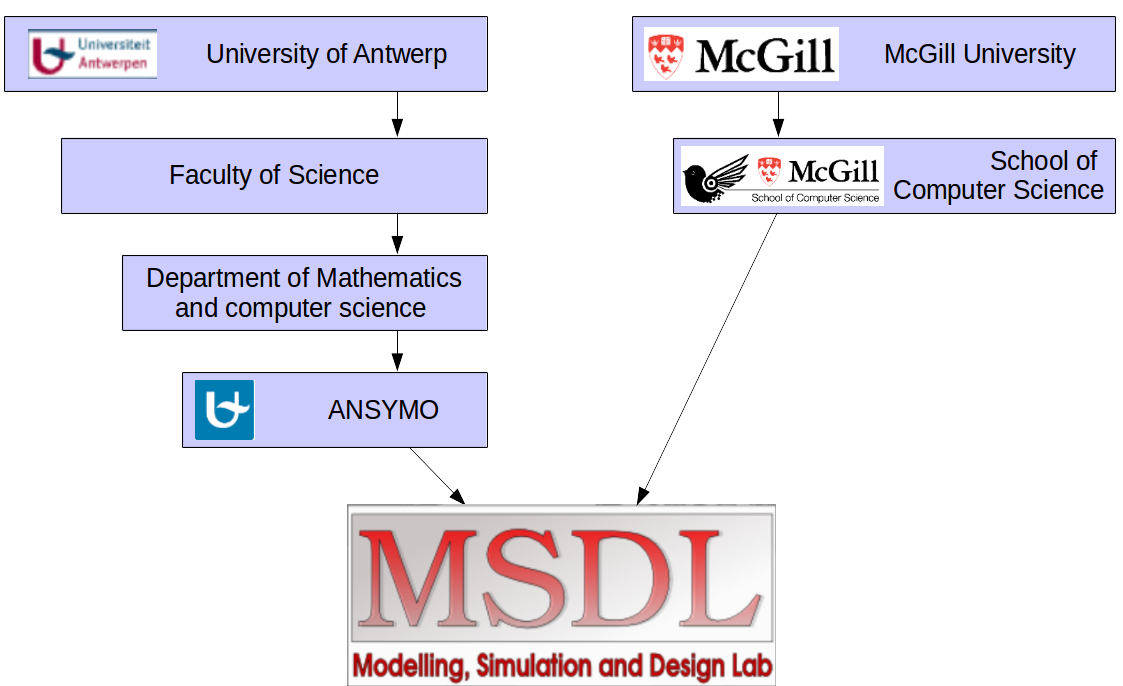
\includegraphics[width=0.8\linewidth]{msdl_organisation}

  \caption{Position of MSDL}
  \label{fig:msdl_org}
\end{figure}

The MSDL laboratory have members in two school, most part of these members are in the University of Antwerp but there is also some PhD students in the McGill University. McGill University is an English-language public research university in Montreal, Canada. You can see on the figure \ref{fig:msdl_org} a description of the organization of these universities\footnote{Only departments which belongs msdl were presented} and the position of MSDL in this organization.


\section{Description of MSDL}


\begin{figure}[!h]
  \centering
  
\includegraphics[width=0.6\textwidth]{MSDLbanner}
  \caption{MSDL banner}
  \label{fig:msdl}
\end{figure}


\begin{quotation}
<<The Modelling, Simulation and Design lab (MSDL) headed by Prof. Hans Vangheluwe is part of the School of Computer Science of McGill University in Montreal, Quebec, Canada and of the AnSyMo (Antwerp Systems and software Modelling) group in the department of Mathematics and Computer Science of the University of Antwerp, Antwerp, Belgium. The MSDL has projects, researchers and students in both locations.>>\cite{msdl}
\end{quotation}


So MSDL is a laboratory of Modeling. It is an important field of computer science because that could permit to create an engineering language understandable by everybody because it is based on graphical diagram. That also permit to create software without programming, just with logical diagram. I had the opportunity during my internship to participated in a presentation of all research subject. The figure \ref{fig:subject} is a not exhaustive list of all research topics discussed in MSDL. The part the most in connection with my subject was \textit{Simulation} and \textit{Analysis, Validation, Verification, Testing, and Accreditation} for obvious reasons.


\begin{figure}[h]
  \centering
  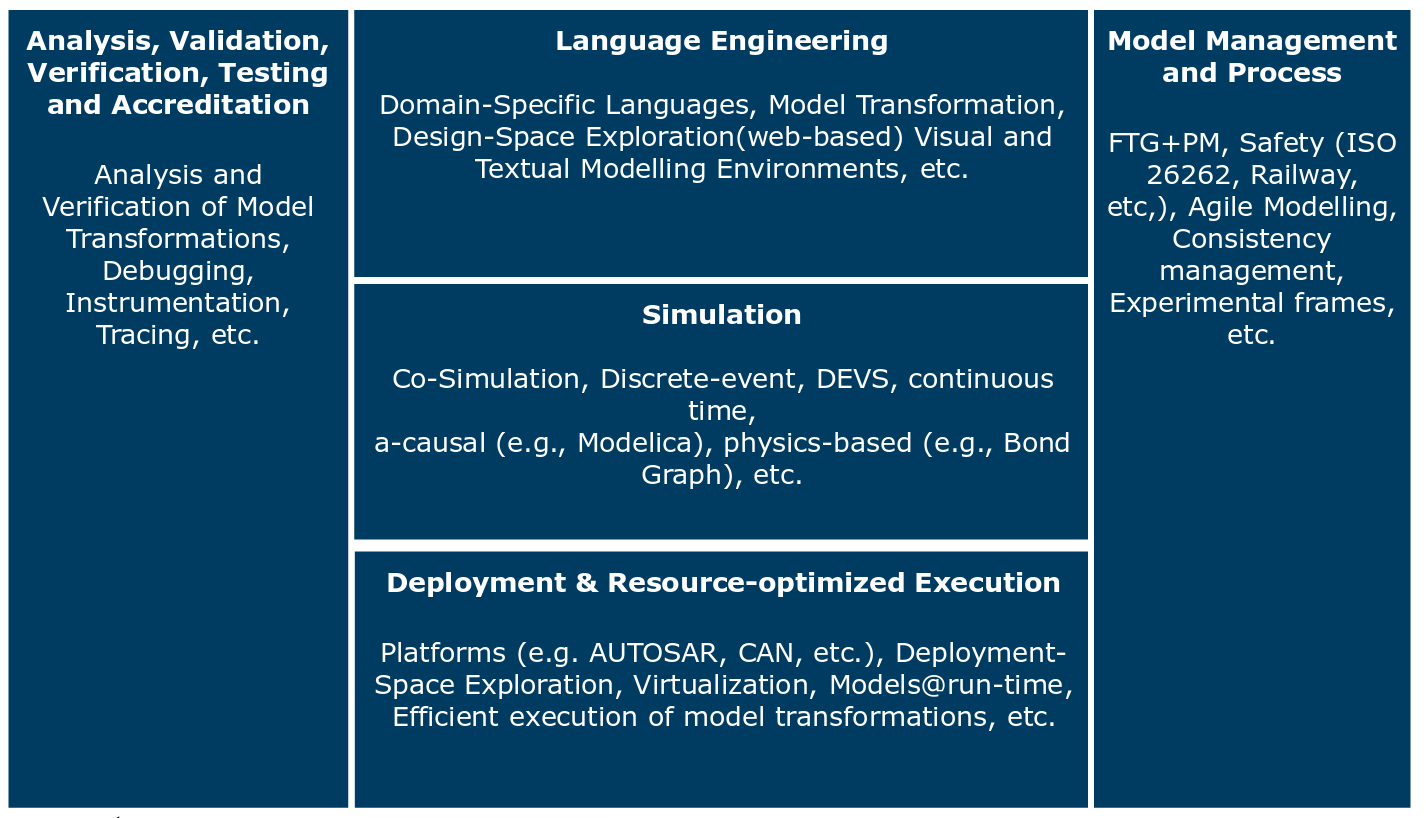
\includegraphics[width=\linewidth]{research}
  \caption{Research topics}
  \label{fig:subject}
\end{figure}



%%% Local Variables:
%%% mode: latex
%%% TeX-master: "../rapport_de_base"
%%% End:



\part{Presentation of the project}


\chapter{Issues}
\label{chap:issues}


As it was explain in the introduction, the issue of this project is to propose a visualization of UML Model for \umld.

\section{Short term issue}

In short term, this plugin should permit at Mr. Champeau and Mr. Teodorov to use during their classroom \umld as an free alternative and multi-platform of Rhapsody with all their interesting feature. In this way, every student could install on their own computer the tool use in classroom.

Advantages of \umld compare to Rhapsody: free, open source, work on Windows, Linux, and Apple.

\section{Long term issue}

Because this plugin is open source and downloadable on a Git Server\footnote{\url{https://msdl.uantwerpen.be/git/michael/UML-DSimulator}}, it will be use by everybody. My hope is this plugin will be improve by the community, student, teacher, \etc... and became a serious alternative to Rhapsody and Papyrus simulator.

~\\

  \begin{figure}[h]
    \begin{minipage}{0.45\linewidth}
      \centering
      
\includegraphics[width=0.7\textwidth]{Rapsody}
      \caption{Rational Rhapsody}
      \label{fig:rhapsody}
    \end{minipage}\hfill
    \begin{minipage}{0.45\linewidth}
      \centering
      
\includegraphics[width=\textwidth]{Papyrus}
      \caption{Papyrus}
      \label{fig:papyrus}
    \end{minipage}
  \end{figure}


%%% Local Variables:
%%% mode: latex
%%% TeX-master: "../rapport_de_base"
%%% End:

\chapter{The plans of the project}
\label{chap:goals}

\section{Definition of my project}

After some interview with Mr. Champeau, I define the table of requirements (tabular \ref{tab:requirements}). This table contains all requirements define by the client to respect the issues of this project define before.

\textit{FS} means service function and \textit{C} means constraints.

\noindent{}
\begin{table}[!h]
  \centering
  \begin{tabular}[h]{|m{0.2\linewidth}|m{0.25\linewidth}|m{0.45\linewidth}|}
    \hline
    \multicolumn{3}{|c|}{Table of requirements}\\
    \hline
    Number&Type of Designation&Designation\\
    \hline
    FS1&UI&Represent the visualization in the UML Model with graphical tools\\
    \hline
    FS2&UML Designer&Works by default this the Ciprian simulator\\
    \hline
    FS3&Simulator&Have the possibility to change the simulator with an other simulator, for example SCCD\\
    \hline
    FS4&Simulation&Give some debugging tools, for example play, stop, \etc...\\
    \hline
    C1&License&Open Source\\
    \hline
    C2&Compatibility&Be multiplatform. Works on Linux, Windows, and Apple.\\
    \hline
    C3&Documentation&Have documentation, code readable, modularity, etc. In that way, this project could be improved during another internship. \\
    \hline
    C4&User&Be user-friendly\\
    \hline
  \end{tabular}
  \caption{Table of requirements}
  \label{tab:requirements}
\end{table}

Then, it is also possible to represent the project with a octopus diagram (figure \ref{fig:octopus}). This diagram permit to show the interaction with the outside world that the client expected.

\begin{figure}[!h]
  \centering
  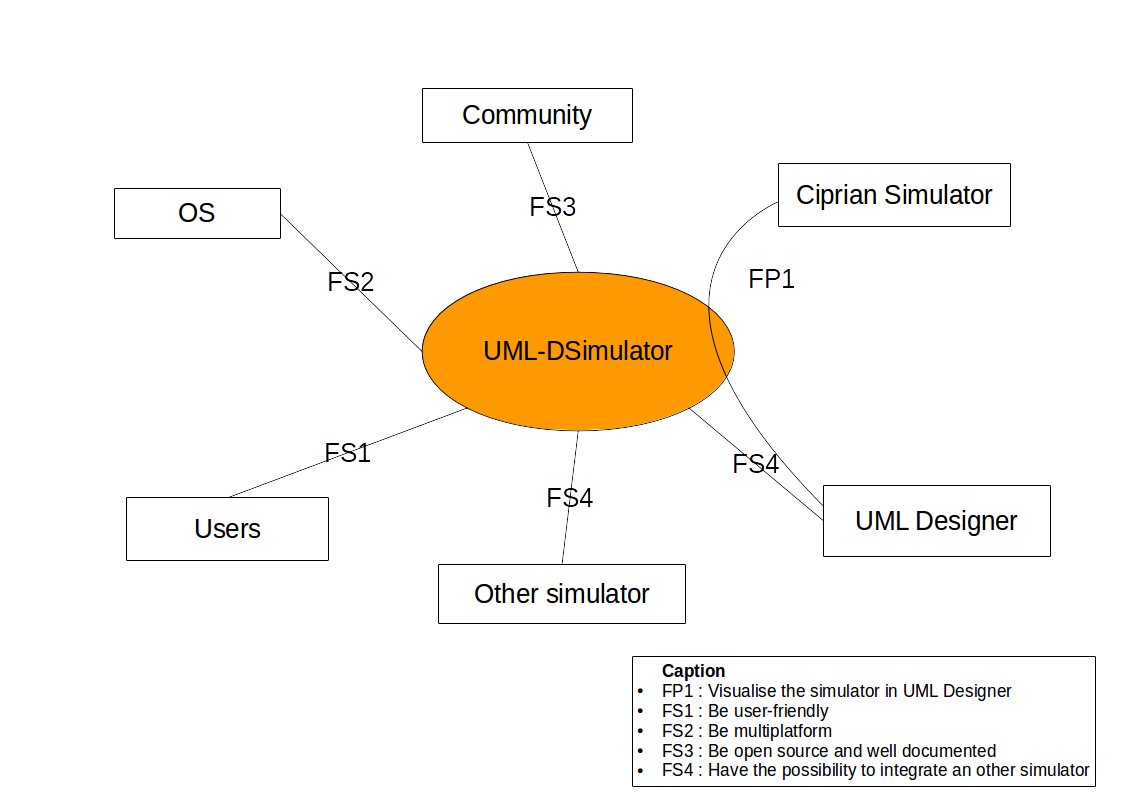
\includegraphics[width=\textwidth]{pieuvre}
  \caption{Octopus diagram}
  \label{fig:octopus}
\end{figure}

\newpage
\section{Goals}

As it was explain in the introduction, the main goal of this project is integrate a simulator in UML Designer. To do that Mr. Ciprian put at my disposal his own Simulator. So it is possible to describe my goals in this order:

\begin{enumerate}
\item Find the way to add plugin in \umld, and understand how it is possible to add some feature.
\item Understand how work the Ciprian simulator.
\item Find a way to integrate the simulator but keep the possibility to change it. Moreover it should be kept in mind that the simulator was not finish so the integration of the simulator need to preserve modularity.
\item Propose some debugger tools. For example: a play button, a stop button, \etc.
\item Write documentation and comment in the code to be reusable. Mr Champeau wanted to keep the choice to do some improvement after the end of this internship.
\item Try an other simulator and compare its performance with the Ciprian simulator.
\end{enumerate}





% \section{Solution proposed}

% After this definition of the goals and the requirements,

% The main goal of this project is to visualize a simulation of Statechart in UML Designer. The simulator should permit to visualize and debug a model of a state machine. Moreover, UML Designer is a modeling software for UML model and Statechart, so we could create the model and simulate it on the same tools.


% The picture \ref{fig:project} represent the aim of this project.

% \begin{figure}[h]
%   \centering
%   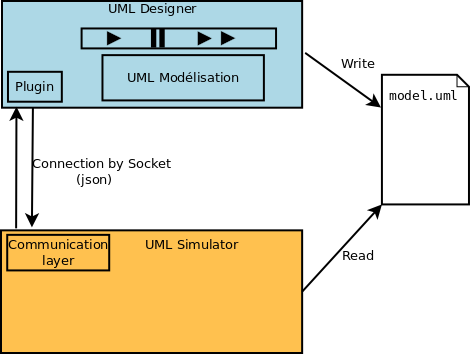
\includegraphics[width=\textwidth]{project}
%   \caption{Description of the project}
%   \label{fig:project}
% \end{figure}







\section{Tools at my disposal}

It is a short description of \umld and the Ciprian Simulator. A further description can be found in the appendix \ref{chap:UMLDesigner} and \ref{chap:simulator}.
\newpage
\subsection{\umld}
\begin{figure}[!h]
  \begin{minipage}[h]{0.45\linewidth}
    \centering
    
\includegraphics[width=0.6\textwidth]{logo}
    \caption{UML Designer logo}
    \label{fig:logo}
  \end{minipage}\hfill
  \begin{minipage}[h]{0.45\linewidth}

    At the beginning of this project, some tools were at my disposal. First of all, it was \umld created by the french company \textit{Obeo}. It is an open source software documented so I could download the source and work on it. It is a UML modeler with a user interface. It is based on Eclipse and Sirius. It follows the UML2 standard which is know and documented.

  \end{minipage}
\end{figure}


\subsection{Simulator}
\begin{figure}[!h]
  \begin{minipage}[h]{0.45\linewidth}

    Then, Mr Ciprian Teodorov, one of my professor, has developed a simulator for UML Model. This simulator needed to be improved, but it composed a good beginning for this project.

  \end{minipage}\hfill
  \begin{minipage}[h]{0.45\linewidth}
    \centering
    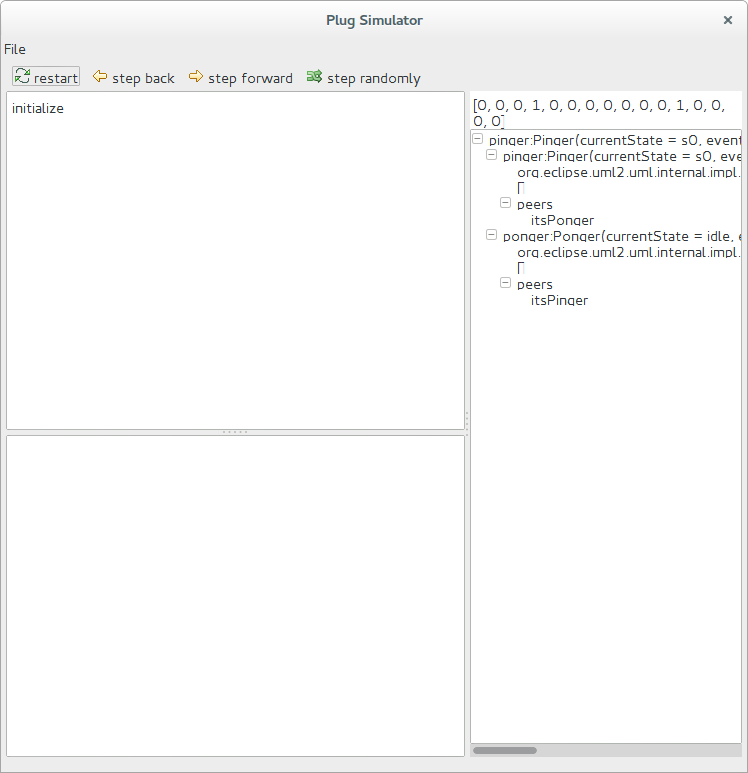
\includegraphics[width=0.9\textwidth]{simulator}
    \caption{Mr Teodorov simulator}
    \label{fig:sim}
  \end{minipage}
\end{figure}







%%% Local Variables:
%%% mode: latex
%%% TeX-master: "../rapport_de_base"
%%% End:


\chapter{Organisation of the work}





%%% Local Variables: 
%%% mode: latex
%%% TeX-master: "../rapport_de_base"
%%% End: 


\part{Results of the internship}


\chapter{Communication inter process}

\section{Type of communication conceivable}

A lot of type of communication inter process were suggested to create a discussion enter the plugin and the simulator. But we will present only the most consistent.

The communication is the part the most important of this project, because that will implement the interface between the two software.

\subsection{Socket}

\begin{tabular}{|p{0.45\textwidth}||p{0.45\textwidth}|}
\hline
  \textbf{Advantages}&\textbf{Drawback}\\
\hline
Work with every simulator type (python, java, ...) & communication synchronous\\
\hline
\end{tabular}

\subsection{File}

\begin{tabular}{|p{0.45\textwidth}||p{0.45\textwidth}|}
\hline
  \textbf{Advantages}&\textbf{Drawback}\\
\hline
Problem when two software want to change the same file at the same moment& Communication asynchronous\\
\hline
\end{tabular}

\subsection{Named pipe}

\begin{tabular}{|p{0.45\textwidth}||p{0.45\textwidth}|}
\hline
  \textbf{Advantages}&\textbf{Drawback}\\
\hline
It is possible to use the Simulator outside the graphical modeling tool & \\
\hline
\end{tabular}


\subsection{Shared Memory}

\begin{tabular}{|p{0.45\textwidth}||p{0.45\textwidth}|}
\hline
  \textbf{Advantages}&\textbf{Drawback}\\
\hline
It is possible to use the Simulator outside the graphical modeling tool & \\
\hline
\end{tabular}


\subsection{Thread}

\begin{tabular}{|p{0.45\textwidth}||p{0.45\textwidth}|}
\hline
  \textbf{Advantages}&\textbf{Drawback}\\
\hline
&Need to recode the simulator \\
\hline
\end{tabular}


\subsection{Our solution}

The solution was not in this list of common way to communicate inter process. In fact, we use the \textit{Runtime} class which is in the java library.~\\


\begin{tabular}{|p{0.45\textwidth}||p{0.45\textwidth}|}
\hline
  \textbf{Advantages}&\textbf{Drawback}\\
\hline
It is possible to use the Simulator outside the graphical modeling tool & \\
\hline
Work with every type of simulator& \\
\hline
\end{tabular}





%%% Local Variables: 
%%% mode: latex
%%% TeX-master: "../rapport_de_base"
%%% End: 


\chapter{The simulator}
\label{chap:simul}

First of all, I worked on the simulator to know specificities of the simulator and realize the layer of communication.

\section{Specificity of the UML Model}

The Ciprian simulator simulate a UML model but this UML model need to have some specificities in the architecture and in the language.

\umld use 2 files to save a uml project. The first is named \textit{model.uml} it contains all UML elements and the declaration of UML diagrams. The second is named \textit{representation.aird}, it contains the specification of the graphical representation.

To work, the simulator need the \textit{model.uml} file. Moreover, this file need to contain some specifics features. It need a class \textbf{SUS} which contain the declaration of all other classes and all other classes need to have a State Machine diagram associated, as you can see on the figure \ref{fig:simulateur}.

\begin{figure}[h!]
  \centering
  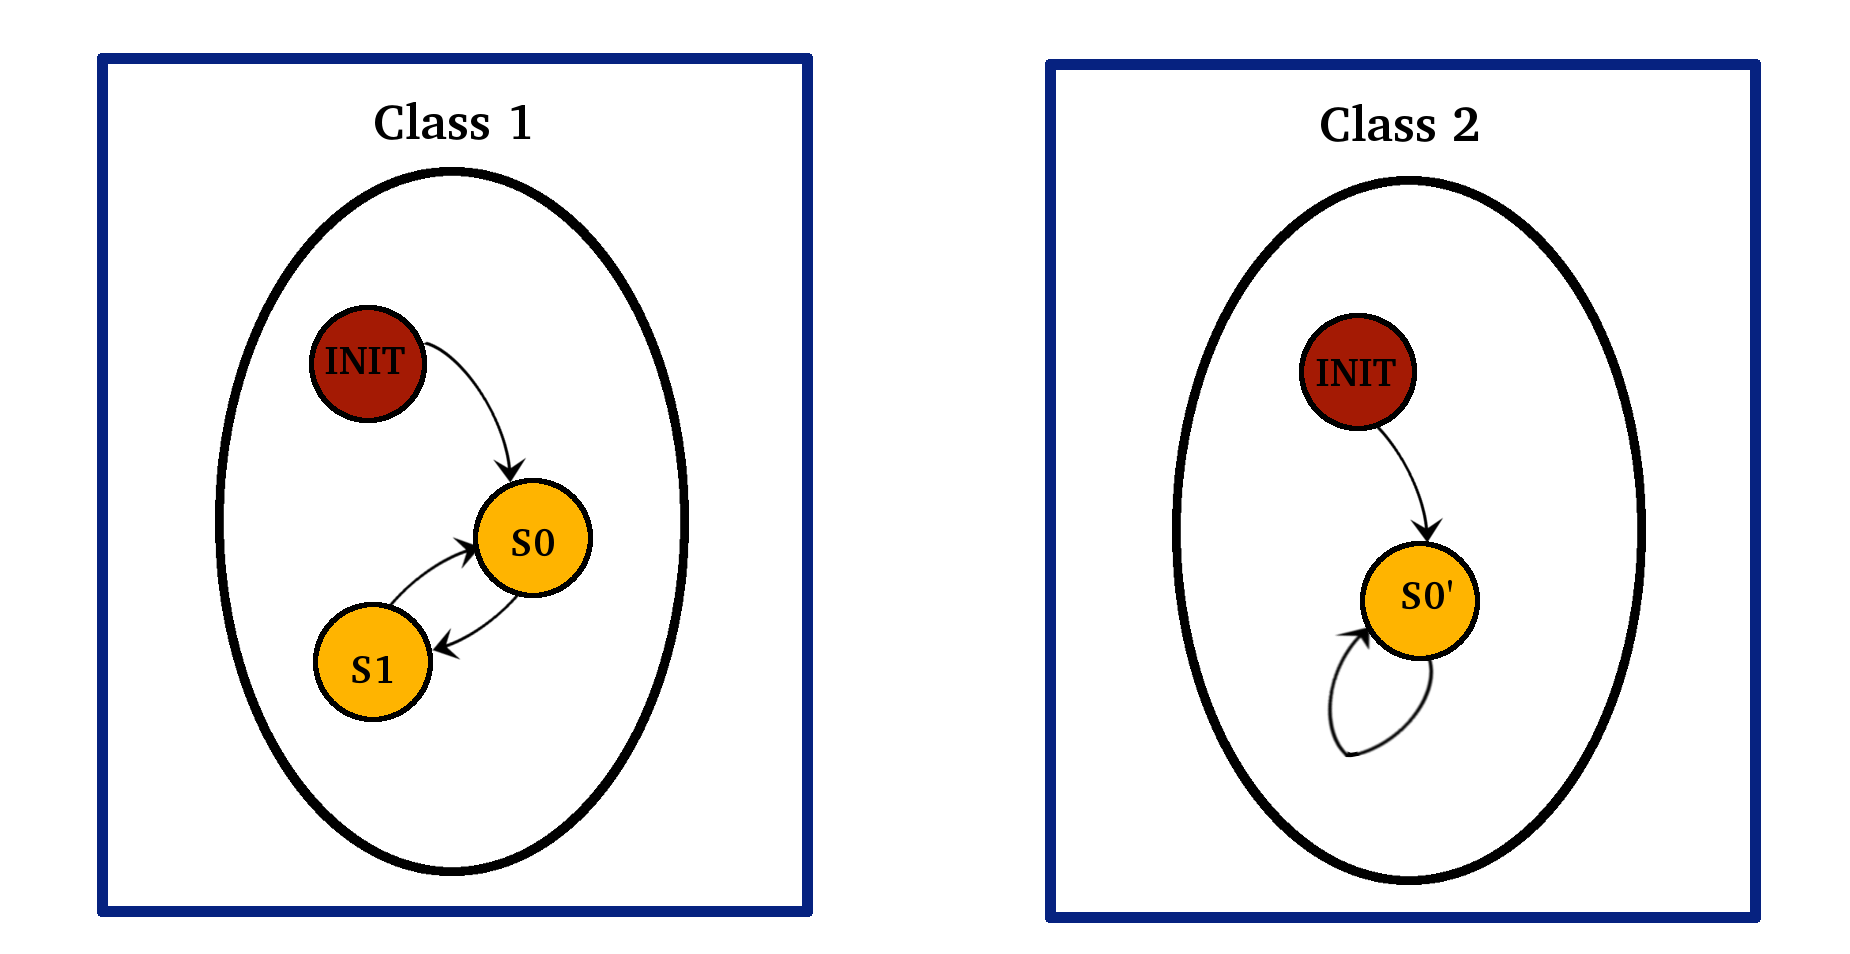
\includegraphics[width=\textwidth]{simulation}
  \caption{representation of the most important elements of the simulator}
  \label{fig:simulateur}
\end{figure}

\section{Additions to Teodorov Simulator}

Afterwards, I made some research on the code of the simulator. I realize that the simulator was not develop to communicate and notify any changing. So I change the code of the simulator to add an Observer pattern at the class \textit{SimulationModel} because this class is a controller of the simulator.

\begin{quotation}
<<The Observer pattern is a software design pattern in which an object, called the subject, maintains a list of its dependents, called observers, and notifies them automatically of any state changes, usually by calling one of their methods.>> \cite{wiki_pattern}
\end{quotation}


I used this pattern to notify the communication class of a changing.

\section{Communication}



The communication Layer was written in Java. In the chapter before, we have decided to put the simulator outside. However, during the implementation we find that is was not very simple to always launch a simulator as a separate software. So I put the simulator and its layer in a new thread inside the plugin. However, the main class of the plugin initiate the Simulator in a new thread and then there is only a communication enter the plugin and the simulator though the localhost loop by socket. Even if the plugin start the simulator thread, we can consider that the simulator is outside because there is no exchange enter this thread without socket.

Moreover, I did some test where the thread is initiate by an other software, and that's work. So for the rest of this report we consider that the simulator is outside the plugin because the comportment is the same, but the default simulator is in fact initiate by the plugin.






%%% Local Variables:
%%% mode: latex
%%% TeX-master: "../rapport_de_base"
%%% End:


\chapter{Plugin}
\label{chap:results}


\section{How to write a plugin}


The first thing that I looked for in the \umld documentation was how add something in the software. It is a real challenge in software development. Fortunately, I quickly found on the \umld developer Guide, that there is a the developer environment to do that. This environment was an Eclipse environment, which is looking as the figure \ref{fig:eclipse}.

\begin{figure}[h]
  \centering
  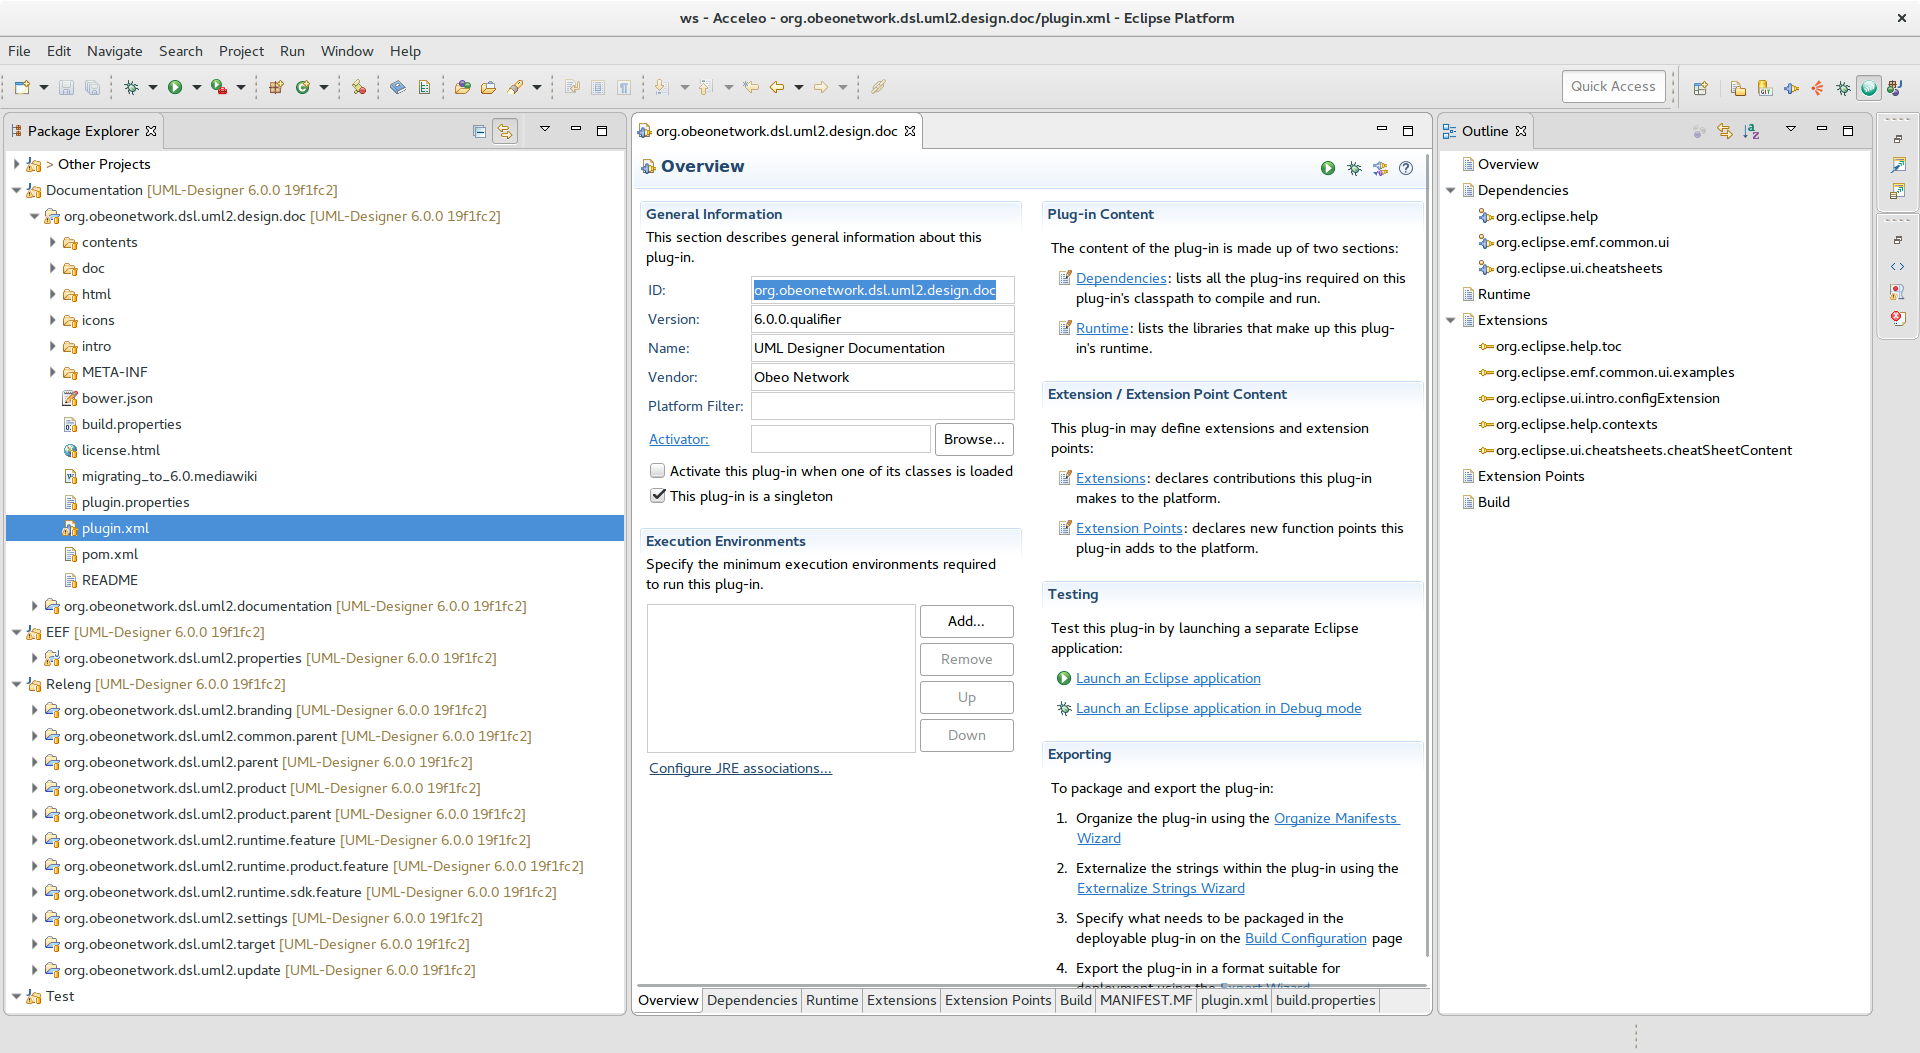
\includegraphics[width=0.8\linewidth]{eclipse}
  \caption{Eclipse environment}
  \label{fig:eclipse}
\end{figure}

Then, I use the fact that \umld is based on Eclipse to create the plugin. The creation of a plugin is the same as an Eclipse plugin. So I made some research on how write an Eclipse plugin. I learn that there is a special structure. This structure permit to keep the modularity and the possibility to install the plugin in all platform. The structure of an eclipse plugin follow the structure show on the figure \ref{fig:plugin}.

\begin{figure}[h]
  \centering
  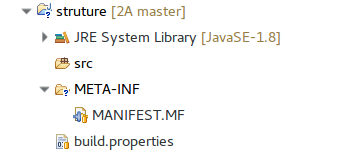
\includegraphics[width=0.5\linewidth]{structure_plugin}
  \caption{Structure of an eclipse plugin}
  \label{fig:plugin}
\end{figure}

\noitemsep
\begin{itemize}
\item The directory \textit{JRE System Library} contains all libraries used to run the plugin
\item The directory \textit{src} contains sources of the plugin
\item The file \textit{MANIFEST.MF} contains addition information for the integration of the plugin
\item The file \textit{build.properties} contains information to export the project
\end{itemize}
\doitemsep

\section{General presentation}

During the development of the plugin, I tried to separate elements of the \umld API, the elements of the UI, and the communication Layer.

The architecture of my plugin follow the UML class diagram presented on the figure \ref{fig:classDiagram}. However, all link enter classes are not represented on it to not overloaded the model. A short description of all sub package:

\noitemsep
\begin{description}
\item[MainView] It is the main class, it is the first class call by \umld when it load the plugin
\item[features] This package contains all graphical elements of the plugins
\item[communication] This package contains the layer of communication of the plugin
\item[tools] This package contains some tools for all class
\item[design] This package contains all classes to change the appearance of the UML Model
\item[model] This package contain a class with all information of the status of the model during the simulation
\end{description}
\doitemsep

Then, it is possible to underline that I use a \textit{Observer} pattern enter classes \textit{MainView} and \textit{CommunicationP} as with the Simulator. This pattern permit to actualize the view of the model when a new communication is received.

\begin{figure}[h]
  \centering
  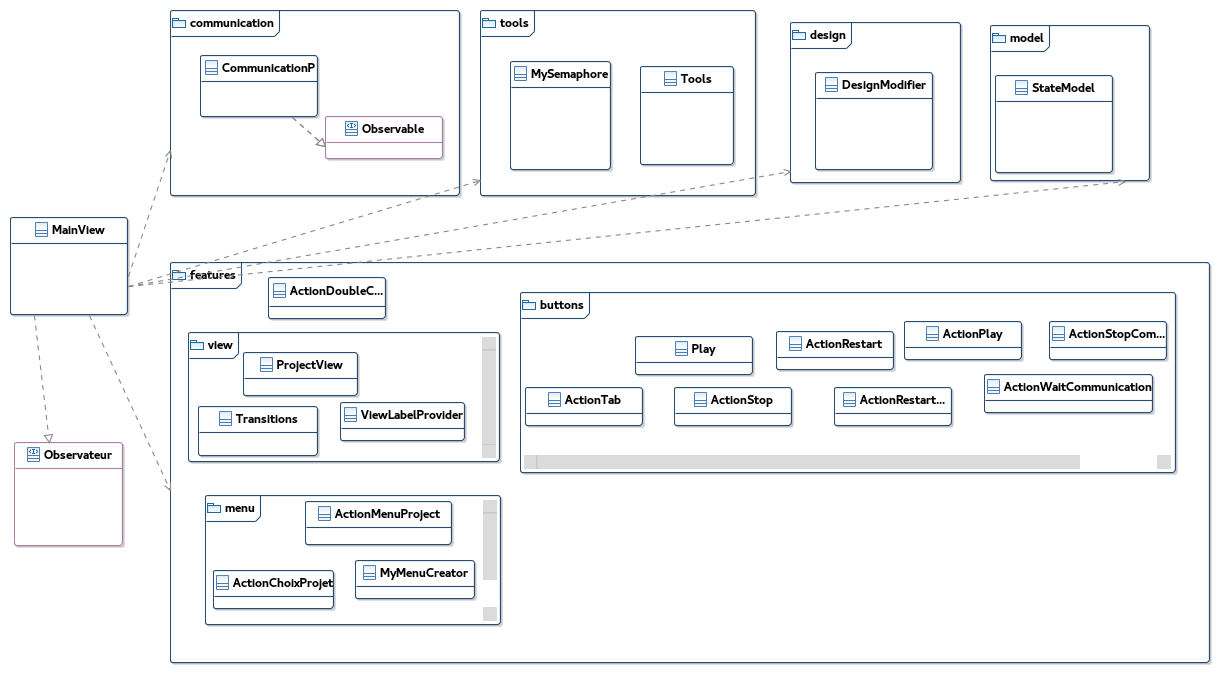
\includegraphics[width=\linewidth]{umlClassDiagram}
  \caption{plugin class diagram}
  \label{fig:classDiagram}
\end{figure}



\section{Functionality implemented}

During this project I had time to implements a lot of functionality for the simulation.


On the figure \ref{fig:result}, you can see the result of my project. It is an Eclipse view, on the top there is a list of all transition possible, and on the bottom it is a tree of the project view. The tree has at the top the name of the project simulated, then the name of all class, end to finish the name of all instances.

\begin{figure}[h]
  \centering
  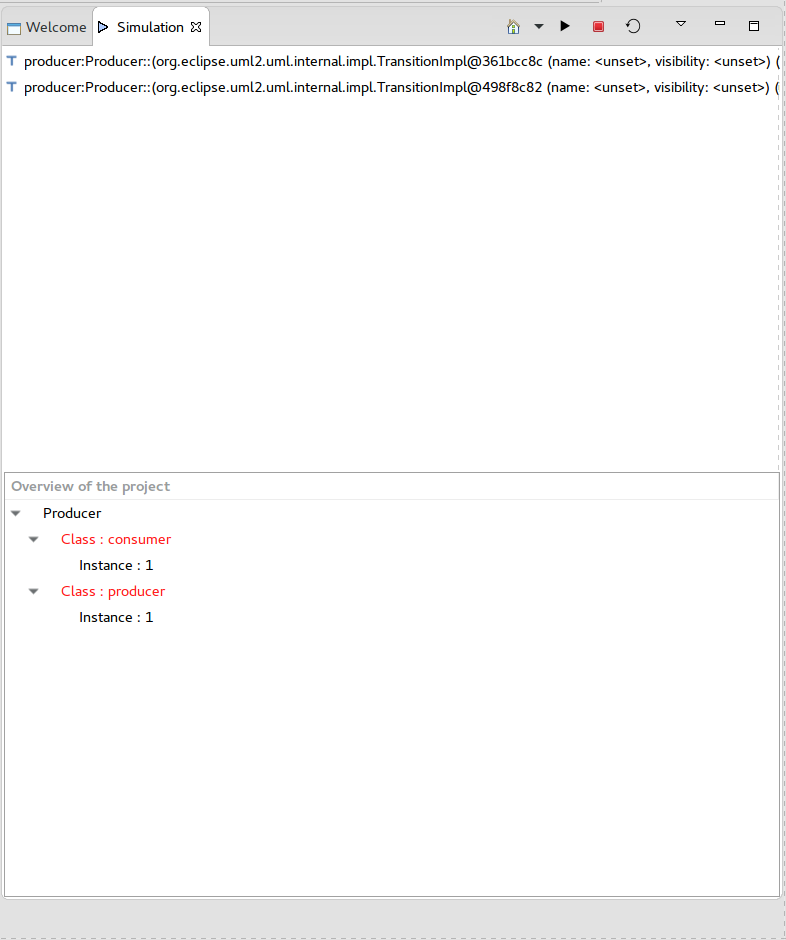
\includegraphics[width=0.4\linewidth]{result}
  \caption{result in \umld}
  \label{fig:result}
\end{figure}

On the top, if the user click on a transition this transition is selected as the next transition, On the bottom, if he click on an instance of a class it is chosen as the visible instance of the model, and if he click on the class name all instances of this class are visible (useful only if there is multiple instance for a same class). Current instances visible are in red.
~\\

On the top, it is possible to see that there is many button. These buttons create some action:

\noitemsep
\begin{description}
\item[home] permit to change the project that we want to simulated
\item[play] launch a simulation where a random step is chosen every 1s.
\item[stop] stop the simulation launch with play
\item[replay] restart the simulation of the project
\item[menu] contain all previous buttons but also:
  \begin{description}
  \item[stop simulator] stop the communication with current simulator
  \item[wait a simulator] start a new server and wait a communication of a new simulator
  \item[restart simulator] restart a communication with the default simulator
  \end{description}
\end{description}
\doitemsep


To finish, I implemented the possibility to see the current state of all state machine diagram in the UML model. You can see on the figure \ref{fig:result2} a test that I did on one model given by Ciprian Teodorov. The red state is the current state.

\begin{figure}[h]
  \centering
  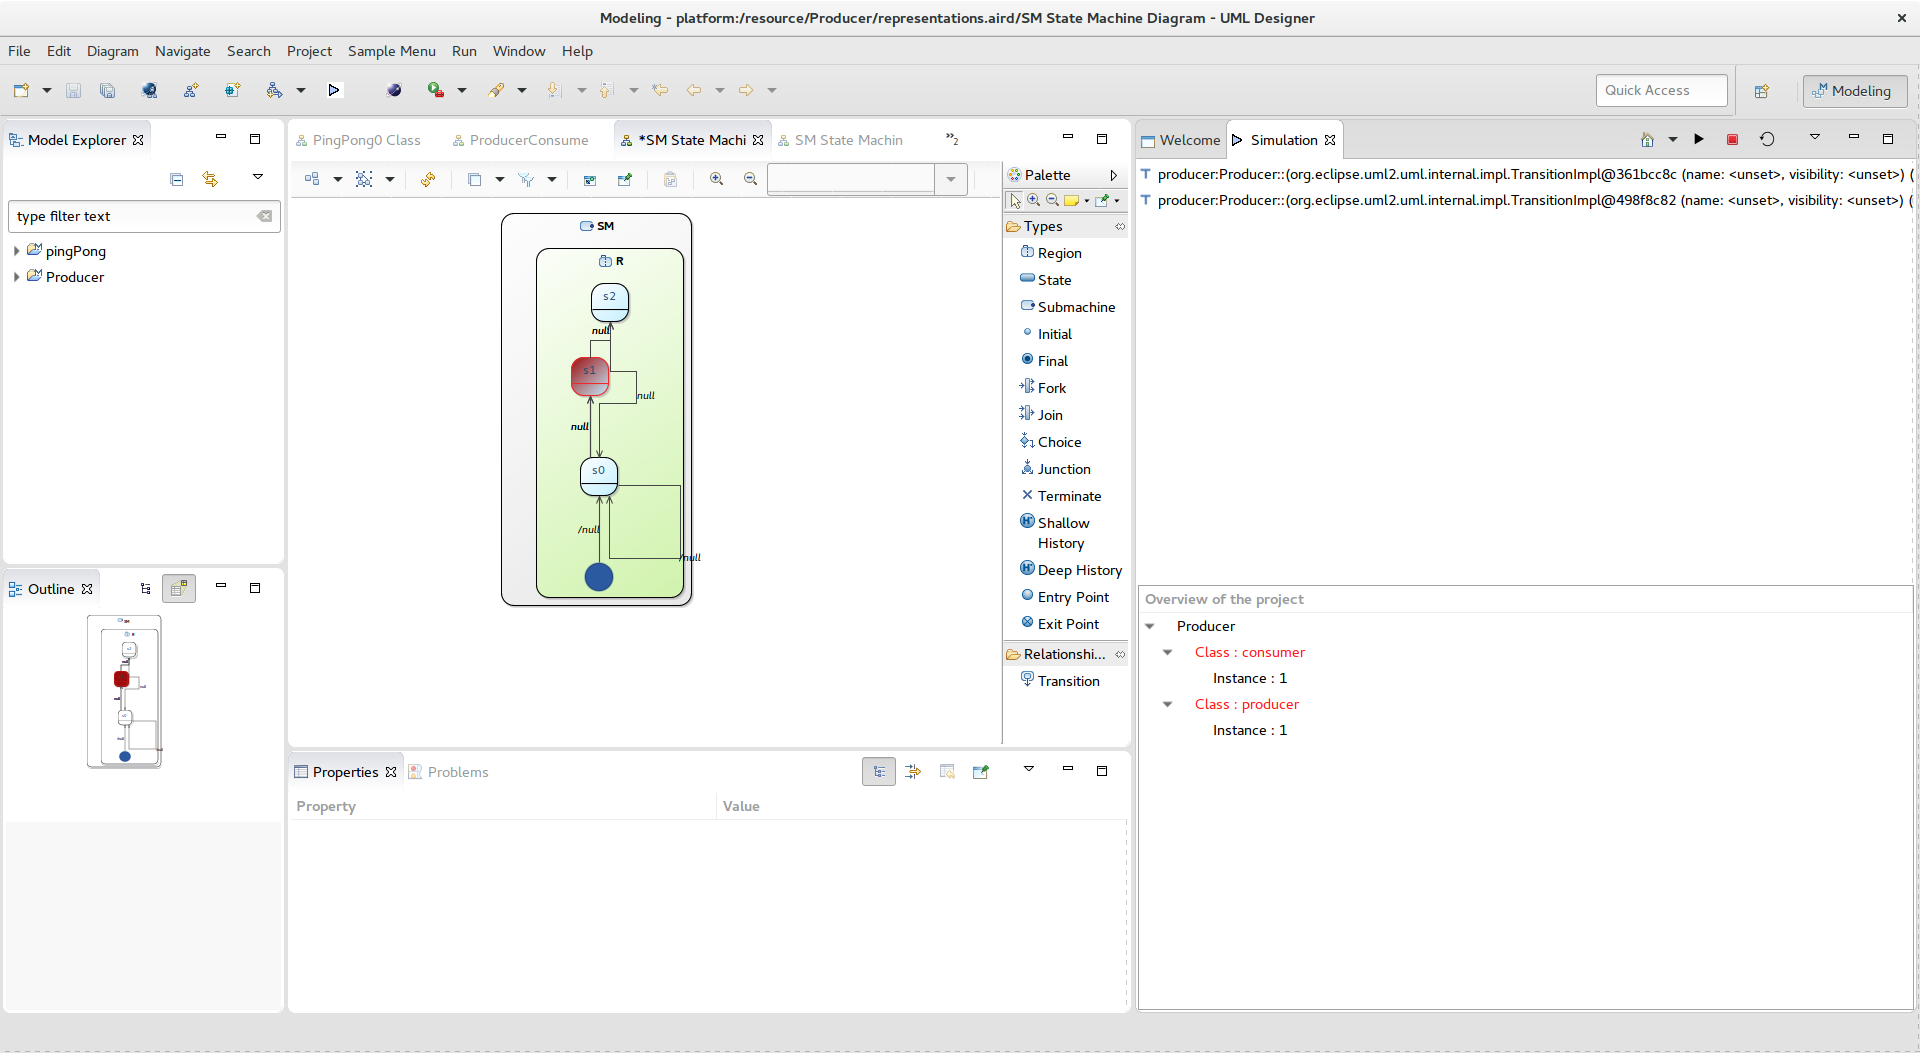
\includegraphics[width=\linewidth]{umldsimulator2}
  \caption{result of a simulation}
  \label{fig:result2}
\end{figure}

~\\

The table \ref{tab:synthese} resume all functionality implemented and also present some functionality suggested during the project but not implemented.

\begin{table}[h]
  \centering
  \begin{tabular}{|p{0.02\textwidth}|p{0.45\textwidth}|p{0.45\textwidth}|}
    \hline
    &Functionality&if not implemented why\\
    \hline
    \hline
    \cmark&Visualization of the simulation in State Machine Diagrams and Class Diagrams&\\
    \hline
    \cmark&Possibility to select the next transition&\\
    \hline
    \cmark&Possibility to change the simulator&\\
    \hline
    \cmark&Possibility to start the simulator outside \umld&\\
    \hline
    \cmark&Possibility to change the current project simulated&\\
    \hline
    \cmark&Possibility to restart the simulation for the current project&\\
    \hline
    \cmark&Play mode (choose a random step every 1s)&\\
    \hline
    \mytilde&Multiple instances for a unique class&The plugin interface take care about multiple instances but the simulator not\\
    \hline
    \mytilde&Parallel state&The plugin interface can show parallel state but it is not implemented on the simulator\\
    \hline
    \xmark&Historical state&It is not yet implemented on the simulator\\
    \hline
    \xmark&Generation of the sequence diagram automatically&Not enough time\\
    \hline
    \xmark&Select the next transition on the UML Model&Not enough time\\
    \hline
    \xmark&Show multiple instances in multiple tabs&Make the project too heavy\\
    \hline
    \xmark&Choose a state for debugging&Not enough time\\
    \hline
  \end{tabular}
  \caption{Functionality implemented}
  \label{tab:synthese}
\end{table}

% I am going to present the result of my work. If you want a better description of the problems and the choice taken you can read the appendix ???.


% \section{Plugin}

% First I will talk about the plugin. The plugin is the part which realize the display in \umld and the communication to the layer of the simulator. \umld is based on Eclipse so to realize the plugin I realize a Eclipse plugin.
% ~\\



%%% Local Variables:
%%% mode: latex
%%% TeX-master: "../rapport_de_base"
%%% End:


\chapter{SCCD}
\label{chap:sccd}

In this chapter, I will talk about SCCD. In the MSDL laboratory, they use SCCD to simulate Statechart. After a presentation of my project in July, they suggested me to try their simulator and compare it to the Ciprian simulator. There is more explanation about SCCD tools in annex page ???.

\section{Transformer}

As we see before, the project has been written to have a ability to change the simulator. However, the model need to be written in scxml standard to be interpreted by SCCD. So the first things that I have to do is a transformer in XSLT. XSLT is a language for transforming XML documents into other XML documents.
~\\

After some research on the internet I found only one transformer written by apache on Github\cite{apache}. The last commit of this project was in 2009, so we can assume that the project is abandoned. I had tried to use it but it didn't work. For this reason I have created a new transformer, but I used some part of this project.
~\\

My transformer have the ability to transform a xmi file as a scxml file. However, model given by my professor had some specificities so I take care to adapt to its.

For example, when there is a script in ABCD language and the script is <<send eventA to itsPinger>> the translation in the state machine is <<raise eventA to itsPinger>>. Then I use the fact that our project always have a \textit{SUS} class which contains all other classes, so in the scxml model the \textit{SUS} class start all other classes.

\section{Utilization}

\subsection{SCCD debugger}

In my project I want to visualize states of all state machine. To do that, I need some informations of the status of the model. SCCD don't permit this type of utilization, but the SCCD debugger written by Simon Van Mierlo can do it.
~\\

However, during my internship this debugger wasn't finished. The debugger can create only one class because the object manager doesn't work.
~\\

To prove that my scxml model created automatically will work when the debugger will be finished, I tried to do a prove of contest. %I use my scxml model created by my transformer automatically in SCCD and I verify the running.

\subsection{SCCD}

To do this prove of contest, I achieve some tests on the pure SCCD. I use the last version of SCCD published in the beginning of august.


I quickly realize that my model had infinite loop. These loops are explain because in the model there is some state which have transition on itself, and this transitions are always verify. In the Ciprian simulator it was not a problem because the user has to choose the next transition and so he was the condition. To fix this problem I add on these transitions a timer of 1s.

You can see on the figure \ref{fig:sccd} the result of the Ping-Pong example on SCCD. As it was expected there is an event which is send from ping to pong and then from pong to ping.

\begin{figure}[h]
  \centering
  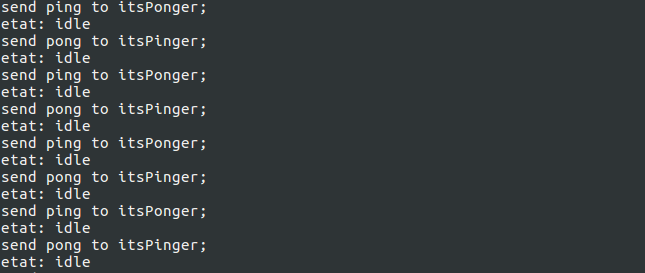
\includegraphics[width=\linewidth]{sccd}
  \caption{pingpong simulation on SCCD}
  \label{fig:sccd}
\end{figure}


%%% Local Variables:
%%% mode: latex
%%% TeX-master: "../rapport_de_base"
%%% End:


\chapter{Tests}
\label{chap:test}

\section{Unit tests}

During this project I did some unit tests to preserve the code during the development. But, I had a lot of difficulties to tests user interface features, so I chose, on Simon advice, to don't tests them. However, the architecture of the plugin clearly separates UI code from essentially functionalities, which where tested.
~\\

To do this unit tests, I used junit and an eclipse feature EclEmma which permit to see the coverage of code during unit tests. On the Figure \ref{fig:coverage}, you can see the result of the coverage show by EclEmma about my project.
~\\

First of all, you can see the package json was not well tested. This package was written by stleary\cite{json}, so I assumed it was already well tested.

Then, packages org.ensta.uml.sim.views.features and org.ensta.uml.sim.views.design only contain class which do action on the user interface. So I didn't tests them.

After this remarks, it is possible to notice that I tested more then 80\%\footnote{It is the usual value of acceptable coverage} of the code use in other classes.


\begin{figure}[h]
  \centering
  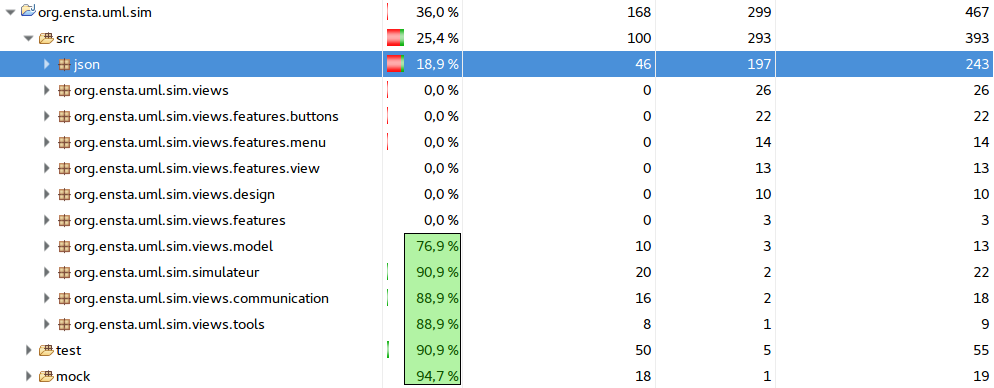
\includegraphics[width=\linewidth]{coverage}
  \caption{Coverage view of my project}
  \label{fig:coverage}
\end{figure}

\section{Integration tests}

I also did some integration tests to verify that the plugin runs in all major platforms (Windows, Linux, Apple).

During all my project I verified that my plugin could be use on my own computer without the eclipse developer environment. I have a Ubuntu 16.04 LTS.

Then, at the end of my project, I tried to use this plugin on other platform. To do that, I use virtual machine with VirtualBox. I tested on a Windows virtual machine with W7 (Figure \ref{fig:windows}), and a Kali virtual machine based on Debian (Figure \ref{fig:kali}). However, I didn't try on OSX because I didn't find a OSX machine.

\begin{figure}[h]
  \centering
  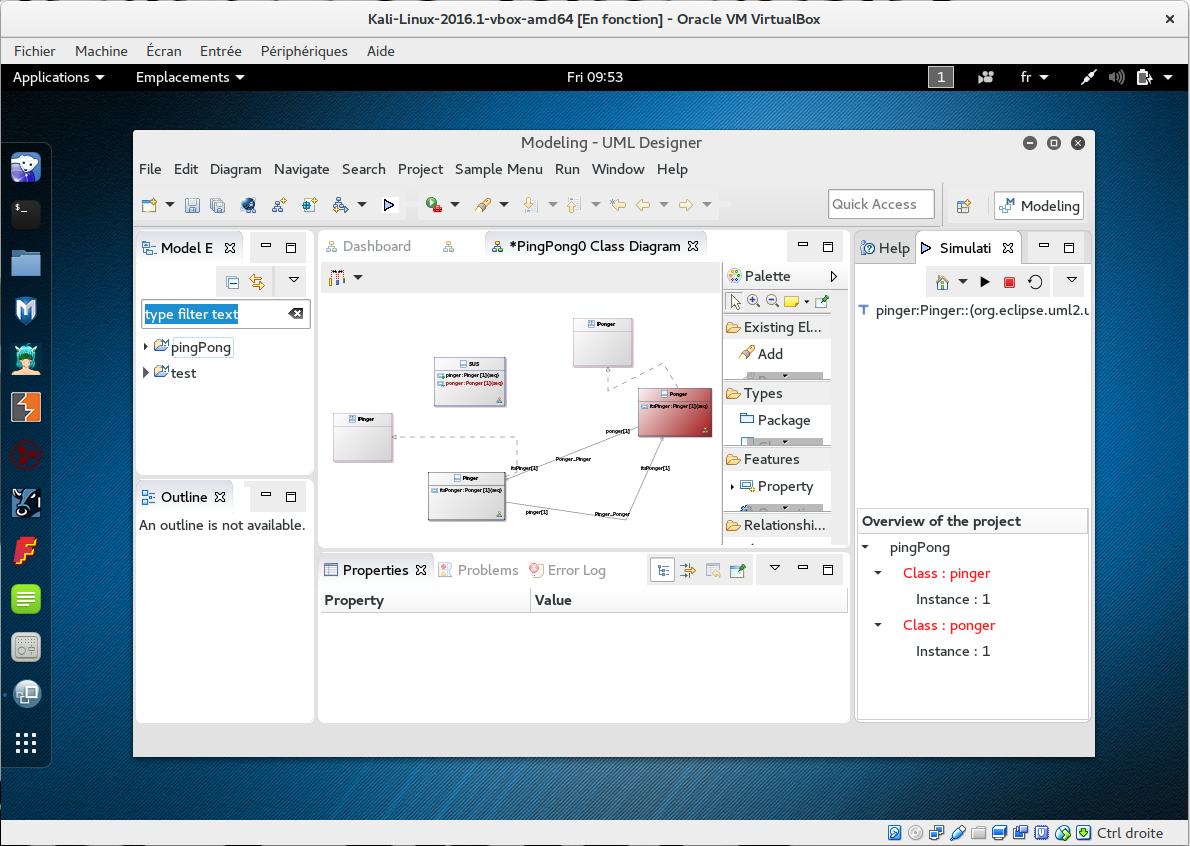
\includegraphics[width=\linewidth]{kali}
  \caption{Screen-shot of the kali virtual machine}
  \label{fig:kali}
\end{figure}

\begin{figure}[h]
  \centering
  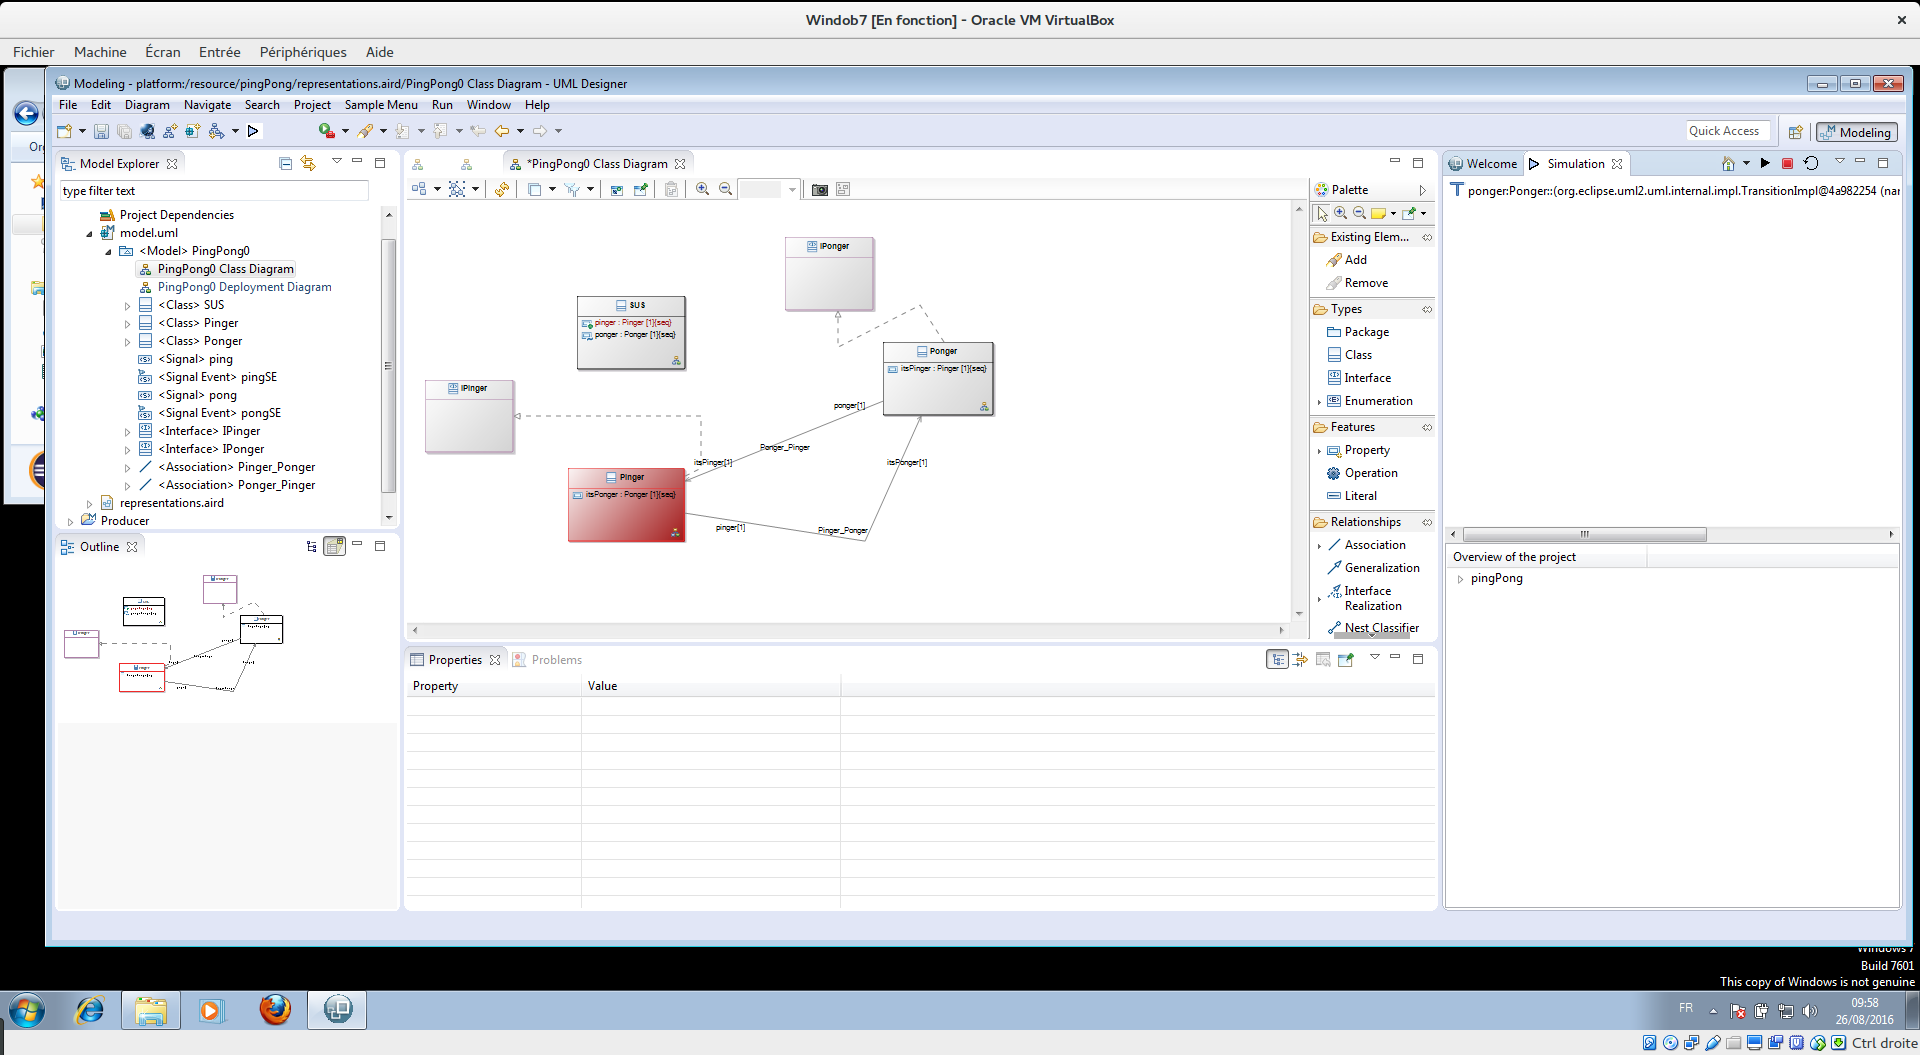
\includegraphics[width=\linewidth]{windows}
  \caption{Screen-shot of the Windows virtual machine}
  \label{fig:windows}
\end{figure}


%%% Local Variables:
%%% mode: latex
%%% TeX-master: "../rapport_de_base"
%%% End:

% \input{Partie/UI}


\part{Contribution of this internship for my professional project}

\chapter{Professional and personal balance sheet}

\section{Profits from this experience}

\subsection{The acquisition of new technical skills}

During this internship I have discovered new technical skills, and I have consolidated skills acquired at ENSTA Bretagne. My project was developed in Java, and I choose to use a managing tools Framaboard (to create Kanban board) and a version control system Git. I understand better why it is important to use this type of tools. Framaboard was very important to keep an overview of my target and keep in mind the task that I have to implement after. Git was very useful to keep track of my work.

Moreover, my work has allowed me to better understand Statechart. In fact, my only experience at ENSTA Bretagne with Statechart was through UML, but during my internship I follow some presentation about Statechart and I try to use SCCD which is a simulator of Statechart.



\subsection{The discovery of a research center}

During this internship I discover the operation of a research center. Even if I will work for the DGA\footnote{Direction générale de l'armement} which is different of a research center, It was very interesting to discover how it works.

I had the opportunity to see some Master Thesis presentation, and follow an introduction of all MSDL researches. It gave me the possibility to better understand their research on Modeling and why they are important.


\section{Encountered difficulties}

During this internship I meet one of the most common problem in software development: the problem of integration. In fact, for me it was very difficult to find a API\footnote{Application Programming Interface} to do action on \umld. In fact, \umld is based on Sirius, EMF, and the Eclipse Kernel, so I had to understand their API to interact on the user interface of \umld. It was very difficult, because when I wanted to do something I had first to find on which API I had to be connected and then how use it.
~\\

An other problem was that the simulator given by Mr Teodorov was stable but not finished. In fact, this simulator has some constraints which block the advanced of new abilities. For example, This simulator doesn't take care about instances. It is a real problem because in OOP\footnote{Object-Oriented programming} there is often object which are instantiated several times. Even if, my plugin was written to have the possibility to show multiple instances, it was not possible to test it on real model.



%%% Local Variables:
%%% mode: latex
%%% TeX-master: "../rapport_de_base"
%%% End:


%%%% CONCLUSION %%%%%%%%%

\chapter*{Conclusion}
\addcontentsline{toc}{chapter}{Conclusion}

I made my project called UML-DSimulator. This project is a plugin for \umld to simulate UML Models.
This project was written to work with the Ciprian Simulator. Currently, the plugin show on the UML Model a visualization of the simulation, give some debugger tools, and have the ability to take an other simulator. However, this plugin was only tested with the Ciprian Simulator which is not finished, and this simulator impose many constraints. %For example, a project need to have a \textit{SUS} class which contains all other classes. This is not an optimal operating.

So, I did a plugin stable and modular which do what Mr Champeau expected, but this plugin is not adapted for the UML community because of the constraints of the simulator. Furthermore, It is possible to notice that this plugin need some improvement especially in the field of debugging.

Despite this, I am very happy because this internship give me the possibility to learn new technical skills, to overwhelm myself, and to use in a real project managing tools that I learn during my scholarship. Then, I am very proud of my works, because at the end of this internship Mr Champeau seems to be satisfied.
\newpage
%%%% ANNEXE %%%%%%%%%%%%

\part*{Appendix}
\addcontentsline{toc}{part}{Annexe}
\appendix
\chapter{\umld}
\label{chap:UMLDesigner}


\umld is an open-source tool to edit and visualize UML2 models created by the French company:
\textit{Obeo}. The project is licensed under the EPL\footnote{Eclipse public license}

\begin{figure}[h] \centering
  
\includegraphics[width=0.3\textwidth]{logo}
  \caption{UML Designer logo}
  \label{fig:logo}
\end{figure}

\section{Utilization}

\umld is a graphical modeling tool for UML2 as defined by OMG\footnote{Object Management Group\cite{omg}}. As
you can see on the figure \ref{fig:umldesigner}, it permit to create diagram on which ones it is
possible to add some elements. The type of the elements proposed depend on the types of the diagram
chosen. For example, if you choose a \textit{User case diagram} it is possible to add 'user'
component that is impossible in \textit{Class diagram}.

So with graphical action it is possible to create many UML diagram which have transverse elements.

To finish, it is possible to create the code of the application that you have develop from the
model.


\begin{figure}[h] \centering
  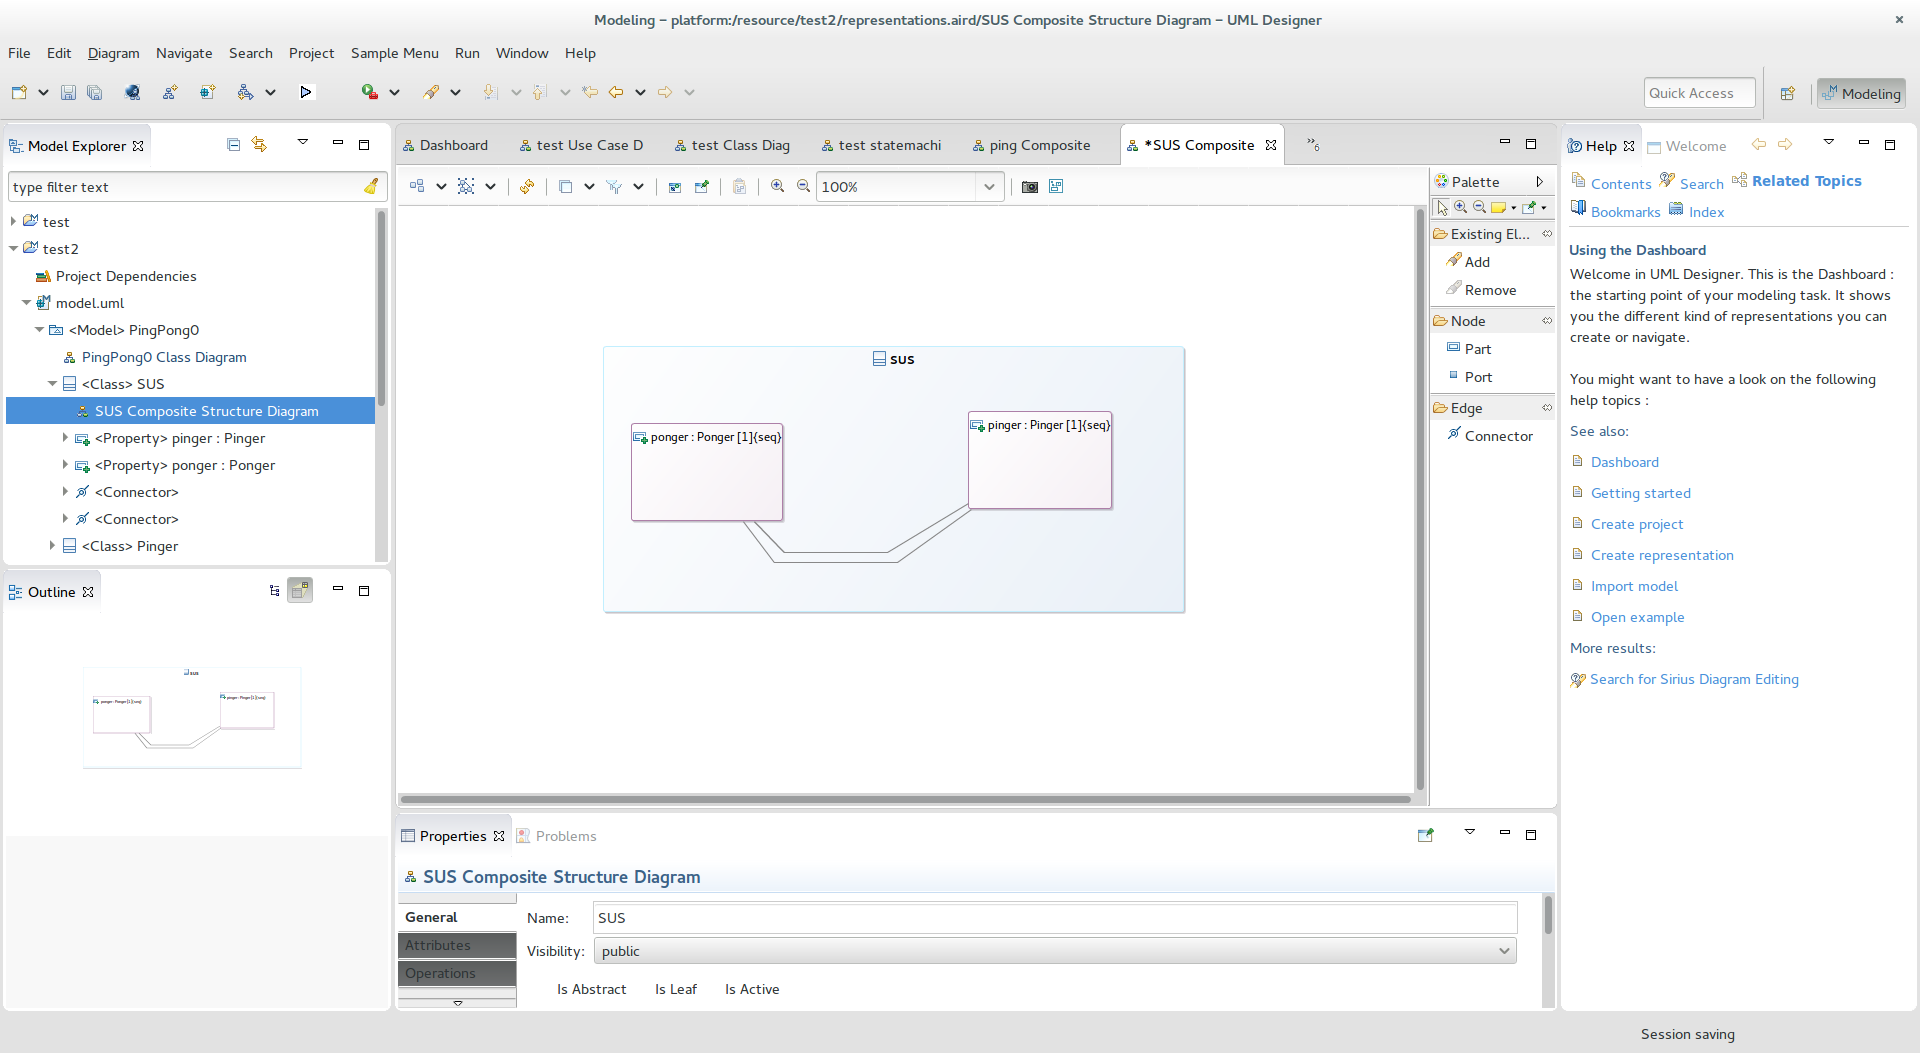
\includegraphics[width=0.8\textwidth]{umldesigner}
  \caption{Screen shot of \umld}
  \label{fig:umldesigner}
\end{figure}



\section{List of diagram supported}

\begin{itemize}
\item Packages diagram
\item Use case diagram
\item Activity diagram
\item Class diagram
\item Component diagram
\item Composite Structure diagram
\item Sequence diagram
\item State Machine diagram
\item Documentation table
\item Use Case cross table
\item Package containment diagram
\item Profile diagram
\end{itemize}



\section{Released}
\begin{center}

  \begin{tabular}{|c|c|}
    \hline
    \textbf{Version} & \textbf{Release Date} \\
    \hline
    1.0.0 &2012\\
    \hline
    2.0.0 &17 January 2013\\
    \hline
    2.1.0 &1 February 2013\\
    \hline
    2.2.0 &12 April 2013\\
    \hline
    2.3.0 &13 June 2013\\
    \hline
    2.4.0 &13 September 2013\\
    \hline
    3.0.0 &17 January 2014\\
    \hline
    4.0.0 &8 July 2014\\
    \hline
    4.0.1 &5 August 2014\\
    \hline
    5.0.0 &29 May 2015\\
    \hline
    \cellcolor{green}6.0.0 &19 October 2015\\
    \hline
  \end{tabular}

  \begin{tabular}{c}
    Legend:\\
    \cellcolor{green}Latest stable release\\
  \end{tabular}

\end{center}

\section{Base on}

\umld is based on a Eclipse and Sirius. It is a UML2 Eclipse plugin.

\subsection{Sirius}
Sirius is an open-source software project of the Eclipse Foundation. Sirius allows to create graphical modeling workbench. It include EMF\footnote{Eclipse Modeling Framework} and GMF\footnote{Graphical Modeling Framework}. On the figure \ref{fig:sirius}, it is possible to see the architecture of Sirius.


\begin{figure}[h]
  \centering
  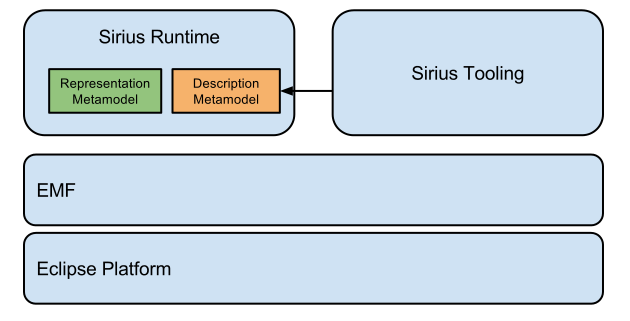
\includegraphics[width=\textwidth]{sirius_archi}
  \caption{Sirius architecture\cite{sirius}}
  \label{fig:sirius}
\end{figure}

\subsection{Eclipse}

\umld is base on Eclipse. 
The interface is the same as Eclipse. You can notice on figure
\ref{fig:umldesigner} that the menu are the same in the both software.



\begin{figure}[h] \centering
  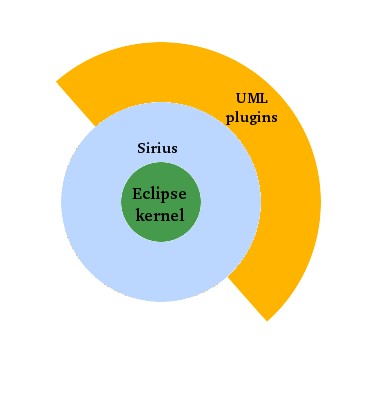
\includegraphics[width=0.5\textwidth]{archi}
  \caption{The \umld kernel}
  \label{fig:kernel}
\end{figure}






%%% Local Variables:
%%% mode: latex
%%% TeX-master: "../rapport_de_base"
%%% End:


\chapter{Simulator}

\section{Description}


At the beginning of this project, we had at our disposal the simulator of Mr Teodorov (figure \ref{fig:sim}). This simulator have a graphic user interface as you can see on the figure \ref{fig:sim}.


\begin{figure}[h]
  \centering
  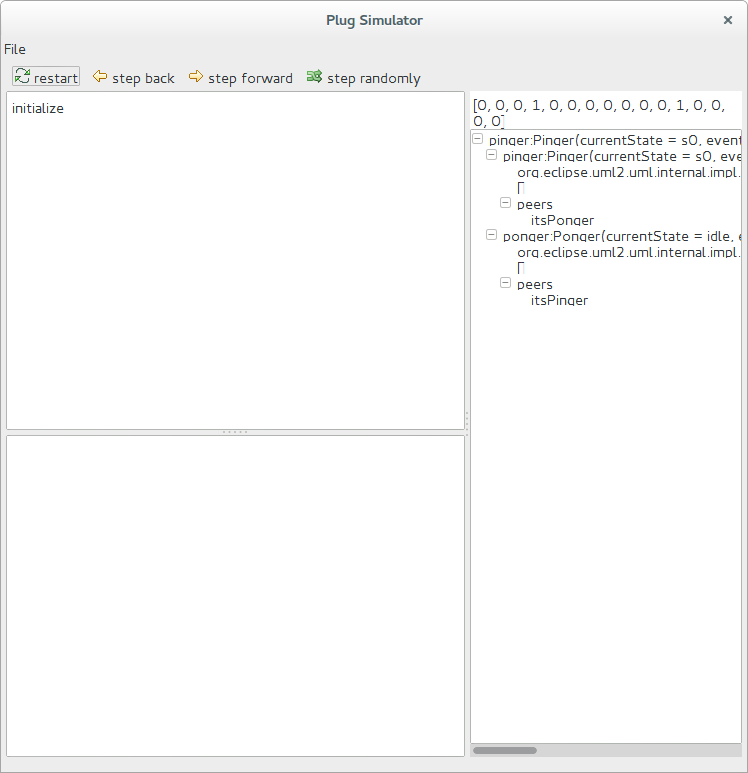
\includegraphics[width=0.5\textwidth]{simulator}
  \caption{Mr Teodorov simulator}
  \label{fig:sim}
\end{figure}


The simulator is compose on 4 part.
\begin{itemize}
\item On the top: some buttons to select an action
\item On the top-left-corner: The list of the next step
\item On the bottom-left-corner: The State Machine associated to the Current State.
\item On the right: A visualization of the Statechart
\end{itemize}

\section{Specificity of the uml file}

This simulator simulate a uml file. The uml file need to have a particular architecture.

\umld to save the uml project use 2 files. The first is named ``model.uml'' and the second is named ``representation.aird''.

To work, the simulator need the \textit{model.uml} file. Moreover, this file need to contain some specifics feature. It need a class \textbf{SUS} which contain the declaration of all other classes and all other classes need to have a State Machine diagram associated. You can see on the figure \ref{fig:simulateur}, that all classes need to have their own State Machine diagrams.

\begin{figure}[h!]
  \centering
  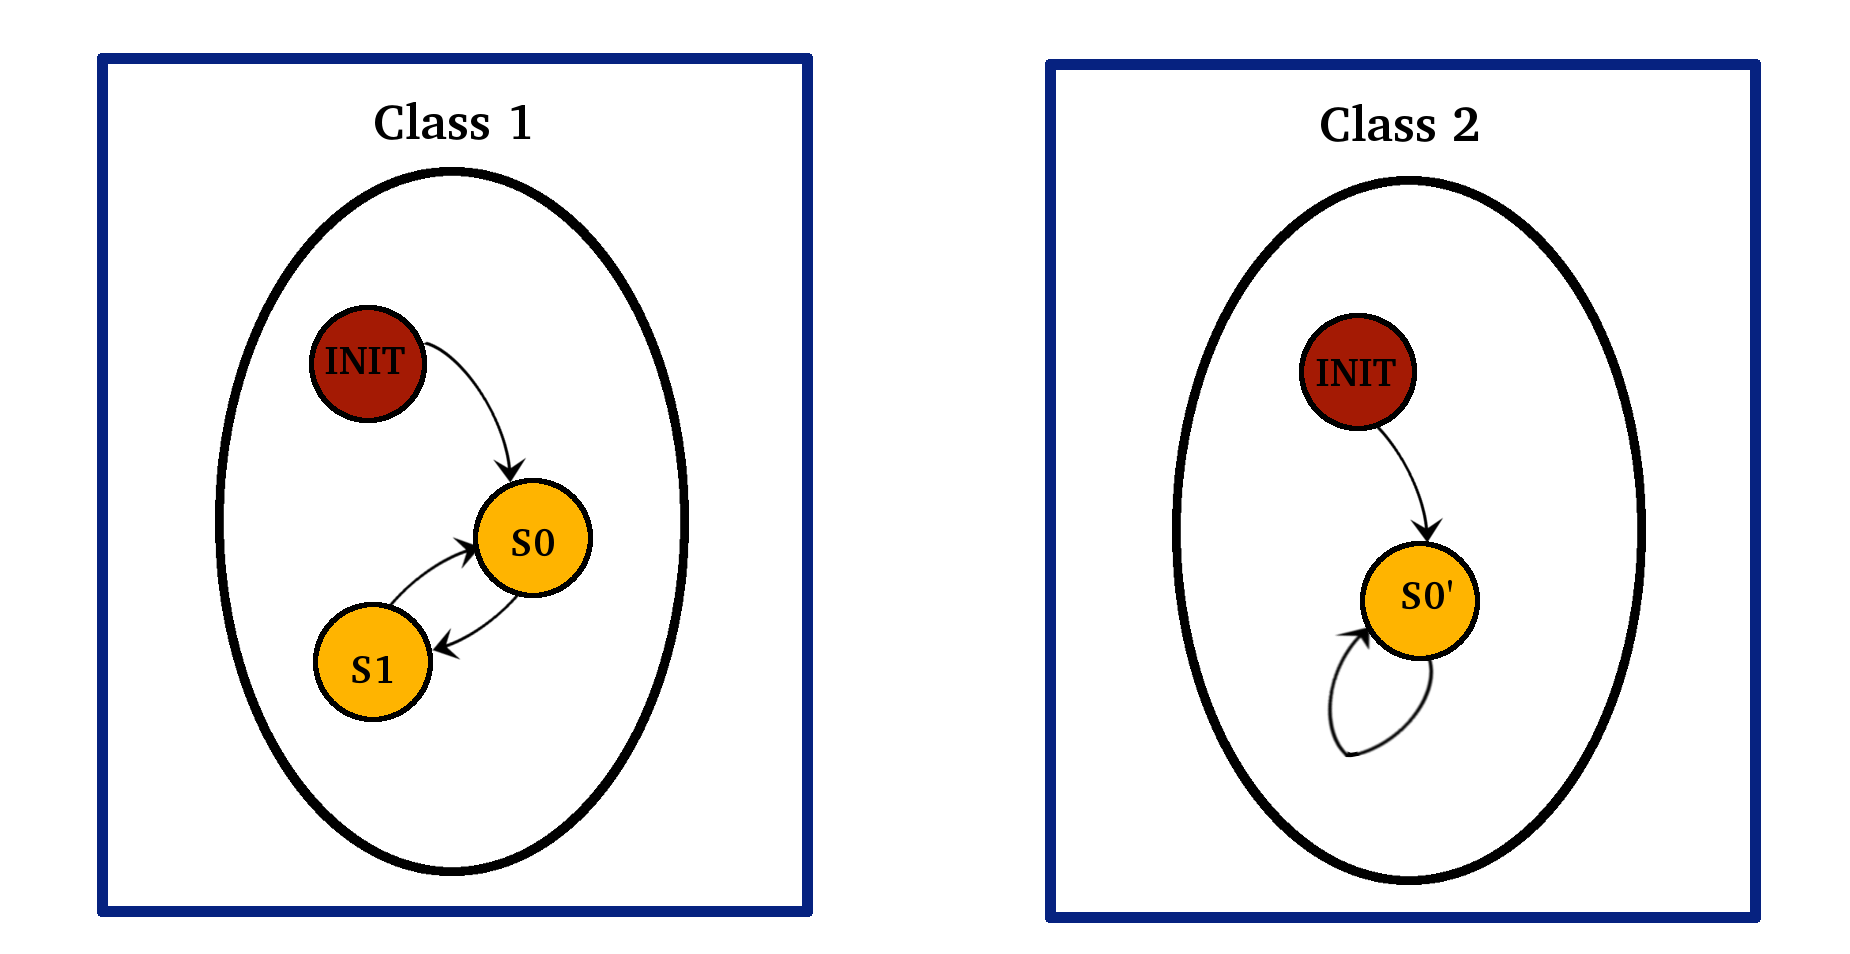
\includegraphics[width=\textwidth]{simulation}
  \caption{representation of the most important elements of the simulator}
  \label{fig:simulateur}
\end{figure}




%%% Local Variables:
%%% mode: latex
%%% TeX-master: "../rapport_de_base"
%%% End:


\chapter{Inter-process communication}
\label{annex:choice}


We are only interesting in communication which permit to exchange data and synchronize them. There is a short presentation of all other communication considered.

\section{Message queue}

\begin{tabular}{|p{0.45\textwidth}||p{0.45\textwidth}|}
\hline
  \textbf{Advantages} & \textbf{Drawback}\\
  \hline
  Work on most operating systems & The implementation depends on the OS\\
  \hline
  One part don't need to know the other &\\
  \hline
  No serialization/deserialization & \\
  \hline
  Very fast&\\
  \hline
\end{tabular}
~\\

The main problem is that the implementation depends on the OS, that is why we don't chose this communication.



\section{Pipe}

\begin{tabular}{|p{0.45\textwidth}||p{0.45\textwidth}|}
  \hline
  \textbf{Advantages}&\textbf{Drawback}\\
  \hline
                     &All POSIX systems, Windows\\
  \hline
                     &The implementation depends on the OS\\
  \hline
                     & Windows: Only one-way pipes (Anonymous pipe and Named pipe\cite{windows})\\
  \hline
\end{tabular}
~\\

This drawback is to penalizing, for the multiplatform constraint.

\section{Message parsing}

\begin{tabular}{|p{0.45\textwidth}||p{0.45\textwidth}|}
\hline
  \textbf{Advantages}&\textbf{Drawback}\\
\hline
&Used only in RPC, RMI, and MPI paradigms, Java RMI, CORBA, DDS, MSMQ, MailSlots, QNX, others\\
  \hline
                     &Slow and complex\\
  \hline
\end{tabular}
~\\

This drawback is to penalizing, for the multiplatform constraint.

% \section{File}

% \begin{tabular}{|p{0.45\textwidth}||p{0.45\textwidth}|}
% \hline
%   \textbf{Advantages}&\textbf{Drawback}\\
% \hline
% Problem when two software want to change the same file at the same moment& Communication asynchronous\\
% \hline
% \end{tabular}

% \section{Named pipe}

% \begin{tabular}{|p{0.45\textwidth}||p{0.45\textwidth}|}
% \hline
%   \textbf{Advantages}&\textbf{Drawback}\\
% \hline
% It is possible to use the Simulator outside the graphical modeling tool & Only available on POSIX systems, Windows, AmigaOS 2.0+\\
% \hline
% \end{tabular}

% \section{Socket}

% Details on the chapter \ref{chap:choice}.

% \section{Signal}

% \begin{tabular}{|p{0.45\textwidth}||p{0.45\textwidth}|}
% \hline
%   \textbf{Advantages}&\textbf{Drawback}\\
% \hline
%  & not usually used to transfer data\\
% \hline
% \end{tabular}


% \section{Shared Memory}

% \begin{tabular}{|p{0.45\textwidth}||p{0.45\textwidth}|}
% \hline
%   \textbf{Advantages}&\textbf{Drawback}\\
% \hline
% It is possible to use the Simulator outside the graphical modeling tool & \\
% \hline
% \end{tabular}




% \section{Our solution}

% For this project we chose to use socket enter the plugin and the simulator. So we need to create a layer of communication for the simulator and a layer of communication for the plugin. Both layer will listen on a thread.

% The solution was not in this list of common way to communicate inter process. In fact, we use the \textit{Runtime} class which is in the java library.~\\

% \noindent
% \begin{tabular}{|p{0.45\textwidth}||p{0.45\textwidth}|}
% \hline
%   \textbf{Advantages}&\textbf{Drawback}\\
% \hline
% It is possible to use the Simulator outside the graphical modeling tool & \\
% \hline
% Work with every type of simulator& \\
% \hline
% \end{tabular}

%%% Local Variables:
%%% mode: latex
%%% TeX-master: "../rapport_de_base"
%%% End:

%\input{Partie/SCCD_complement}
% 
\chapter{SCCD}
\label{chap:sccd}

In this chapter, I will talk about SCCD. In the MSDL laboratory, they use SCCD to simulate Statechart. After a presentation of my project in July, they suggested me to try their simulator and compare it to the Ciprian simulator. There is more explanation about SCCD tools in annex page ???.

\section{Transformer}

As we see before, the project has been written to have a ability to change the simulator. However, the model need to be written in scxml standard to be interpreted by SCCD. So the first things that I have to do is a transformer in XSLT. XSLT is a language for transforming XML documents into other XML documents.
~\\

After some research on the internet I found only one transformer written by apache on Github\cite{apache}. The last commit of this project was in 2009, so we can assume that the project is abandoned. I had tried to use it but it didn't work. For this reason I have created a new transformer, but I used some part of this project.
~\\

My transformer have the ability to transform a xmi file as a scxml file. However, model given by my professor had some specificities so I take care to adapt to its.

For example, when there is a script in ABCD language and the script is <<send eventA to itsPinger>> the translation in the state machine is <<raise eventA to itsPinger>>. Then I use the fact that our project always have a \textit{SUS} class which contains all other classes, so in the scxml model the \textit{SUS} class start all other classes.

\section{Utilization}

\subsection{SCCD debugger}

In my project I want to visualize states of all state machine. To do that, I need some informations of the status of the model. SCCD don't permit this type of utilization, but the SCCD debugger written by Simon Van Mierlo can do it.
~\\

However, during my internship this debugger wasn't finished. The debugger can create only one class because the object manager doesn't work.
~\\

To prove that my scxml model created automatically will work when the debugger will be finished, I tried to do a prove of contest. %I use my scxml model created by my transformer automatically in SCCD and I verify the running.

\subsection{SCCD}

To do this prove of contest, I achieve some tests on the pure SCCD. I use the last version of SCCD published in the beginning of august.


I quickly realize that my model had infinite loop. These loops are explain because in the model there is some state which have transition on itself, and this transitions are always verify. In the Ciprian simulator it was not a problem because the user has to choose the next transition and so he was the condition. To fix this problem I add on these transitions a timer of 1s.

You can see on the figure \ref{fig:sccd} the result of the Ping-Pong example on SCCD. As it was expected there is an event which is send from ping to pong and then from pong to ping.

\begin{figure}[h]
  \centering
  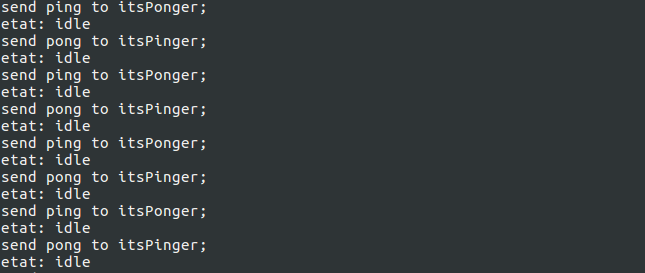
\includegraphics[width=\linewidth]{sccd}
  \caption{pingpong simulation on SCCD}
  \label{fig:sccd}
\end{figure}


%%% Local Variables:
%%% mode: latex
%%% TeX-master: "../rapport_de_base"
%%% End:


\nocite{*}
%\input{annexe_}
\newpage
~\\
\newpage
\listoffigures
\listoftables
 \printindex
 \bibliographystyle{plain}
  \bibliography{biblio}

\end{document}
%%%%%%%%%%%%%%%%% FIN DU DOCUMENT
%%% Local Variables:
%%% mode: latex
%%% TeX-master: t
%%% End:
